\documentclass[12pt]{article} %V1.0
\usepackage{amsfonts,amssymb,amsmath,mathrsfs,amsthm}
\usepackage{graphicx,caption,lipsum}
\usepackage{epsfig,epstopdf}
%\usepackage{harvard}

%\usepackage[margin=2cm]{geometry}
\usepackage[bottom=1in,top=1in,left=1in,right=1in]{geometry}
\setlength{\parindent}{0cm}

%\setlength{\leftmargini}{16pt}

\usepackage[dvipsnames]{xcolor} % en.wikibooks.org/wiki/LaTeX/Colors
\usepackage{enumitem} % bullet points
\usepackage{cmap} % fix the 'fi' problem
\usepackage{rotating,wrapfig,lscape}
\usepackage{bbm}
\usepackage{mathtools} % for multi-lined equations
\usepackage[utf8]{inputenc}
\usepackage[english]{babel}

\usepackage[export]{adjustbox}
\usepackage{setspace}

\onehalfspacing



\newtheorem{theorem}{Theorem}
\newtheorem{corollary}{Corollary}[theorem]
\newtheorem{lemma}[theorem]{Lemma}
\newtheorem{proposition}{Proposition}
 

\linespread{1.25}
\setlength{\parindent}{24pt}



% HYPERLINK
\usepackage[breaklinks=true]{hyperref}
\hypersetup{
  colorlinks=true,
  citecolor=darkblue,
  linkcolor=darkblue,
  urlcolor=darkblue,
  pdfpagemode=none,
  pdfstartview={XYZ null null 1},
  pdftitle={},
  pdfauthor={GH},
  pdfkeywords={} }
\definecolor{darkblue}{rgb}{0,0,0.25}
%

% BIBLIOGRAPHY
\usepackage[longnamesfirst]{natbib}
\bibliographystyle{chicago}
%\bibliographystyle{econometrica}

% DEFINITIONS
\theoremstyle{definition}
\newtheorem{definition}{Definition}%[section]

\captionsetup[figure]{labelsep=period}

\usepackage{palatino}

\setlength{\footnotesep}{1em}

\usepackage{nameref}

\graphicspath{{./figs181014/}}
%---------------------------------------------------------------------------------

\begin{document}

%---------------------------------------------------------------------------------


\noindent {\large \textbf{How much work experience do you need to get your first job? \\ \normalsize The macroeconomic implications of bias against labor market entrants}}   

\vspace{0.6cm}

\noindent \normalsize  \textbf{Shisham Adhikari}

\noindent University of California - Davis

\vspace{0.5cm}

\noindent \normalsize  \textbf{Athanasios Geromichalos}

\noindent University of California - Davis

\vspace{0.5cm}

\noindent  \textbf{Ioannis Kospentaris}

\noindent Athens University of Economics and Business


\vspace{0.5cm}
\noindent This Version: November 2023

%\noindent PRELIMINARY AND INCOMPLETE (DO NOT CIRCULATE WITHOUT PERMISSION)




\vspace{0.7cm}




\normalsize

\noindent ABSTRACT------------------------------------------------------------------------------------------------------
\noindent The first step in a worker's career is often particularly hard. Many firms seeking workers require experience in a related field, so a vicious circle is created, whereby an entry level job is required in order to get an entry level job. Consequently, entrant workers have lower job-finding rates and longer unemployment durations than the unemployed who have looked for a job in the past. To study the welfare implications of these observations, we consider a version of the DMP model where firms who match with entrant workers have to incur training costs. As a result, firms are biased against entrant workers, who, in turn, stay unemployed for a prolonged period of time, exposing themselves to a persistent skill loss shock. In this environment, an obvious market failure arises. Firms who hire entrant workers provide a \textit{benefit to society} by helping these workers stay unemployed for a shorter period of time, thus reducing the probability of skill loss. But since firms cannot internalize this societal contribution, they choose to discriminate against entrant workers causing a welfare loss. We use a calibrated version of the model to quantitatively assess the effectiveness of four government interventions, whose common goal is to reduce bias against entrant workers. We find that the most effective intervention takes the form of a subsidy that induces firms to rank entrants higher than experienced workers.
%an ``internship", where firms can hire entrant workers at an (exogenous) lower wage.      


\vspace{0.4cm}


\noindent JEL Classification: E24, E60, J24, J64

\noindent Keywords: search and matching, unemployment, labor market entrants, training, skills


\vspace{0.6cm}

\noindent \footnotesize Email: shadhikari@ucdavis.edu, ageromich@ucdavis.edu, ikospentaris@aueb.gr.


\thispagestyle{empty}

\noindent We are grateful to Efi Adamopoulou, Marios Angeletos, Andri Chassamboulli, Nicolas Caramp, Miro Gabrovski, Manolis Galenianos, Christos Genakos, Andreas Gulyas, Loukas Karabarbounis, Myrto Kalouptsidi, Minki Kim, Moritz Kuhn, Florian Madison, Guido Menzio, Victor Ortego-Marti, Theodore Papageorgiou, Giovanni Peri, Krzysztof Pytka, Guillaume Rocheteau, Nikos Thedoropoulos, as well as seminar participants at UC Davis, the University of Cyprus, the University of Mannheim, the West Coast Search and Matching Spring 2023 Workshop, the Second Athens Winter Econ Meeting, and CRETE 2023 for useful comments and suggestions.



\newpage
\setcounter{page}{1}
\normalsize

%---------------------------------------------------------------------------------
\section{Introduction}\label{intro} 

    



The first step in a worker's career is often particularly hard. Entrant workers have much lower job-finding rates and longer unemployment durations than the unemployed who have looked for a job in the past (Figure \ref{figure jfr}).
Moreover, positions targeted to workers who have just entered the labor market tend to become a rarity. Indicatively, 35\% of entry level positions posted since 2017 on LinkedIn required years of experience in a related field (see Section \ref{section model discussion}). So a vicious circle is created, whereby an entry level job is required in order to get an entry level job. These observations raise a number of important questions. First, why would firms choose to exclude from the applicant pool workers who are inexperienced, but may turn out to be extremely able? Second, what are the aggregate welfare implications of this bias against inexperienced workers, given that, by definition, \textit{all} workers in the economy start their careers as inexperienced? This last question becomes especially important once we consider the recent literature in labor economics arguing that market conditions during the start of a worker's career have long lasting effects \citep{wachter2020persistent}. Finally, one wonders whether there is room for welfare improving government interventions and what form these interventions should take.  

%It is not clear that firms rank algorithmically (they are flooded with applications and just need some kind of filter even if it is irrelevant to productivity) or something has changed in the nature of production and inexperienced workers have in real terms become more expensive. We could have a version without training costs and algorithmic ranking and provide results.

To study these questions, we augment the classic Diamond-Mortensen-Pissarides (DMP) model in several directions. First, we assume that firms that hire entrant/ inexperienced workers have to incur training expenses. This creates bias against these workers which we capture with a \cite{blanchard1994ranking} matching function with ranking. Second, we assume that entrants who stay unemployed for an extended time period are more likely to suffer skill loss. The combination of these two channels creates interesting welfare trade offs, since the inherent bias against entrant workers increases their unemployment duration which, in turn, tends to lower their productivity. In this environment, an obvious market failure arises. Firms that hire inexperienced workers provide a \textit{benefit to society} by helping these workers stay unemployed for a shorter period of time, thus reducing their exposure to the skill loss shock. (A shock which leaves a permanent ``scar", thus affecting the entrant workers' productivity when they are hired by other firms later in their career.) However, firms cannot fully internalize this societal contribution, and ultimately choose to discriminate against entrant workers, causing a social welfare loss.  

% Source of inefficiency: ranking matching AND nash bargaining

Given this market failure, there is obvious scope for government intervention.
Since the root of the inefficiency is the inability of firms to fully recoup the training costs, which results in hiring bias against entrants, we consider government interventions whose common goal is to alleviate the bias and reduce the inexperienced workers' exposure to the skill loss shock. 
We use a calibrated version of the model to quantitatively study the effectiveness of three government interventions.
The first intervention, which we dub ``unbiased matching'', bans discrimination against inexperienced workers by law.
In the second intervention (``government subsidies''), the government raises taxes to subsidize firms that hire inexperienced workers.
Finally, the third intervention (``internships'') also bans discrimination but additionally explores the possibility that the compensation of entrant workers is determined exogenously by the government.

We find that all three government interventions improve aggregate welfare.\footnote{Some observers would argue that high unemployment rate among entrant workers is a negative thing in its own right based on fairness considerations. Our point, however, is even stronger: we show that policies reducing the unemployment rates of inexperienced workers actually improve the economy's \textit{utilitarian} welfare level.}
This is true even though in all of them the aggregate unemployment rate is higher than in the benchmark economy with ranking.
To explain the economics behind this result, let us begin with the first intervention, i.e. unbiased matching.
Without the ability to discriminate against entrants, firms are effectively forced to incur larger training expenses.
As a result, firm entry is discouraged and equilibrium unemployment is higher compared to the baseline economy.
Despite this unintended consequence on aggregate unemployment, entrant workers have shorter unemployment spells and, as a result, are less likely to suffer skill loss.
The productivity gains from the latter channel are so large that aggregate welfare increases by 0.38\%. %  
The economics behind the second intervention, i.e., government subsidies, is similar, but the welfare increase is smaller (around 0.31\%).
The reason is that the tax needed to finance training subsidies reduces match surplus and further distorts entry.

The third intervention, i.e., internships, achieves all the benefits of the other two, since it also involves unbiased matching, but it suffers less from the downside of discouraged entry. With internships, entrant workers' wages are exogenous and we can treat them as parameters whose level varies.
For high enough wages, entrant workers are compensated almost as much as they would under Nash bargaining and, since ranking is not allowed, welfare levels are close to those of Intervention 1.
On the other extreme, if entrant wages are too low, firms realize they can hire these workers almost for free, which leads to very large levels of training and vacancy creation costs. In total, aggregate welfare has an inverse-U shape with respect to the entrants wage level and it achieves its maximum (0.42\% greater than the baseline) when entrant's wages are at intermediate levels. That is, a carefully designed internship scenario achieves the highest welfare among these interventions.

%Given that these interventions move the equilibrium allocation in the right direction, one wonders to the

The common thread among the interventions considered so far is that they raise aggregate productivity by abolishing bias against entrant workers and, as a result, lowering their exposure to skill depreciation.
In light of this finding, we consider an additional, fourth, intervention, in which the government ``goes all the way'' subsidizing the hiring of entrant workers so heavily that firms actually prefer to match with these workers rather than the experienced ones. 
The results of this intervention are striking: it improves aggregate welfare by 1.4\%, more than three times larger than the internships scenario.
This intervention has the largest impact among all four interventions because it directly confronts the problem of inexperienced workers spending a lot of time in unemployment upon entry.
It should be pointed out that programs that target entrant workers are particularly popular in Europe.
The Youth Employment Initiative, a large EU-sponsored program, directly finances young workers' apprenticeships, traineeships, job placements, and further education within 4 months of leaving school or becoming unemployed.
Our model predicts that interventions of this kind generate sizeable welfare gains.



%After comparing the relative effectiveness of the three interventions, we also examine how close each of them can bring the economy to the constrained efficient allocation, implemented by a social planner who can determine the rate at which different worker types are matched with firms.\footnote{\,In our model, each worker's productivity depends on her experience and on whether she suffered skill loss in her youth. In this environment, setting up the social planner's problem is not completely standard. We think the most meaningful way to do it is to give the planner the tools to address the model's main inefficiency, namely, the bias against inexperienced workers caused by the fact that firms do not internalize the social benefit of hiring (and training) these workers. To that end, we consider a framework where each type of worker searches for firms (and vice versa) in a different submarket. Within each submarket, the social planner must respect the matching process, as is standard. However, the planner has the freedom to choose the number of vacancies in each submarket, which, effectively, allows the planner to choose a different job-finding rate for each worker type. For a detailed discussion, see Section \ref{section planner}.} We find that the social planner achieves 0.81\% higher welfare than the baseline economy (with bias against entrant workers), even though the aggregate unemployment rate, under the constrained efficient allocation, is 21.4\% higher than the baseline economy. The planner achieves this by being able to change the job-finding rates of different worker types, and, specifically, by heavily promoting the hiring of \textit{unscarred} inexperienced workers. The intuition is that the planner fully internalizes the fact that training entrants quickly has large aggregate implications for the economy’s welfare, as it reduces these workers' exposure to the long-lasting skill loss shock. 

%The comparison of the various interventions with the planner's solution provides some important insights. As we saw, all three government interventions increase welfare, but even the most effective one (a carefully designed internship) increases welfare by 0.42\%, which is roughly half of the increase achieved under the constrained efficient allocation. The reason should now be transparent. The interventions we have considered move the equilibrium allocation in the right direction, by abolishing the bias against entrant workers, but the planner's solution reveals that this is not good enough, and that optimality requires that these workers actually match \textit{faster} than other types. Simply put, the socially optimal allocation could be reached only if firms were biased {in favor} of entrant workers. 



The rest of the paper is organized as follows. Section \ref{section model} describes the model, including a discussion of some key assumptions and a literature review, and Section \ref{section analysis} analyzes the baseline model with matching bias against inexperienced workers. Section \ref{section policy interventions} considers three government interventions intended to improve welfare and Section \ref{section calibration} describes the calibration strategy. Section \ref{section results} introduces the fourth intervention and discusses the quantitative effects of all policy interventions considered. Section \ref{section conclusion} concludes. 

%The accompanying Web Appendix analyzes a version of our model where the skill loss shock does not leave a permanent scar. 


%What follows is old notes; most of these have either been incorporated or aborted, but I will leave them here, just in case ?? Thanasis quant exercise: take a newly born (or graduated) worker. Calculate his lifetime utility in a world with bias and in a world where internships are allowed. Conjecture: despite the fact that many people would think that the internship is bad for young workers (cheap labor, slavery and other bs), we may be able to show that the young workers (as well as the whole economy) are better off in the world with internships. 

%?? Thanasis thought on welfare: I had a potentially relevant thought while walking Loki :-) (Everything I will say assumes that there is no ingredient in the model making "excess unemployment among young workers" a de facto bad thing. Later on, we will add such an ingredient, e.g., it could be deterioration of skills or something like that. But recall that for now we want to measure welfare in the plain vanilla model, and then compare it with welfare under the various B specifications to get an idea of the economic channels at work BEFORE we add new ingredients.)  

%If we calculate welfare in the current model(s), the terms $u_0*z_0$ and $u_1*z_1$ will be part of the welfare function. Now, in a world with bias against young workers, $u_0$ will tend to be (relatively) large and $u_1$ will tend to be (relatively) small. Thus, I am conjecturing that welfare in the baseline model (with bias) will tend to be low(er) because a very high value of $u_0$ is a bad thing, as it puts a large weight on the relatively smaller $z_0$ value. Put differently, moving from the baseline model to one of the specifications with policy intervention (2A or 2B or 2C) will tend to improve welfare, as it will lead to a reduction of $u_0$ (which is multiplied by the smaller $z_0$) and in increase of $u_1$ (which is multiplied by the larger $z_1$). (Obviously, there are other things going on in general equilibrium, that's why this is a conjecture.)

%In a sense, our model with $z_0<z_1$ ALREADY (before adding extra ingredients) seems to have a channel whereby an intervention that lowers $u_0$ is a good thing for welfare. Now, that may be good news, but, to be fair, we should not oversell this result or take it too seriously because it is a bit "staged". The various z's should be added into the welfare functions only if we think of them as utility of leisure or home production. BUT if we think of them that way, why on earth is $z_1>z_0$ (why do younger unemployed workers have less leisure or lower home production than experienced ones)? If we wanted to be more careful, here is what we may want to do: we could break the amount that unemployed workers enjoy into a utility term "z" and a (monetary) benefit term "b". The z would be the traditional textbook interpretation of "utility of leisure or home production", and the "b" would be a monetary benefit that the government pays (and to do that they must impose taxes, which, btw is not too hard to deal with; we should eventually do it). 

%Then, what we now call $z_1$ should be: $z_1 = z + b_1$.  And what we call $z_0$ should be: $z_0 = z + b_0$. I could understand why $b_1>b_0$, in fact, I would argue that $b_0 =0$, as we discussed previously! But I think that the utility part of the two expressions, (the "z") should be EQUAL for the two types of workers. Notice that this is important for welfare, because the z's enter the welfare function, but the b's should not (they are transfers from one type of agent to another, they are not utility). 

%In other words, (I think) we want to have a model telling us that some intervention is good for welfare, but we don't want that to happen because of some unreasonable assumption we imposed on $z_0$ and $z_1$. (We want something deeper, like the skill loss or whatever.) 

%---------------------------------------------------------------------------------

\section{The Model}\label{section model}

We consider an extension of the Diamond-Mortensen-Pissarides framework. Time is continuous with an infinite horizon, and all agents discount future at rate $r$. The labor force is normalized to 1. Workers exit the labor market (retire) at Poisson rate $\delta$, and each retired worker is immediately replaced by a new worker, who one should think of as a recent graduate. Naturally, the new workers enter the labor market as unemployed. The retirement of workers, and their consequent replacement by an entrant worker, is crucial in our model, because these new entrants will be a special category, and the length of time they spend being unemployed will have long-term consequences. There is a large mass of \textit{ex ante} homogeneous firms who can enter the labor market with one vacancy. As is standard, the measure of active firms in equilibrium is determined by free entry. 


Firms who decide to enter the labor market and search for workers must pay a flow recruiting cost $c$. Existing jobs get terminated at the job destruction rate $\lambda$. Generally, job matches produce an amount $p$ of the numeraire good, but this productivity will be affected by the worker's specific type, in a way that we now describe. Firms who have hired entrant (inexperienced) workers must pay a flow training cost $\kappa$ until the match dissolves. This is our way of capturing the real world observation that firms are often biased against workers who do not have any working experience. Perhaps these new entrants were brilliant students, but they still need training to become \textit{productive workers}. Thus, one possible interpretation is that the $\kappa$ term is the number of hours other colleagues must spend with the inexperienced workers ``showing them the ropes". (For a further justification of this assumption, see Section \ref{section model discussion}.) After losing their very first job workers become automatically experienced, and firms who shall hire them in the future will not need to pay the $\kappa$ cost ever again.\footnote{\,Our ``training cost" story is not the only way to capture the real world observation that firms are biased against inexperienced workers. Another possibility is that employers have asymmetric information about a worker's quality. The asymmetric information problem would be less severe in the case of a worker who has previously held at least one job, since the firm could ask for a reference letter from a former employer. While our approach is certainly not the only way to go, it has two big advantages. First, it leads to a simple and tractable model. Second, it is extremely relevant and easier to quantify, as there is a large literature studying training costs in the labor market. See Section \ref{section model discussion} for the relevant references.} 


Since the effective productivity of an inexperienced worker is lower than that of an experienced worker (with $\kappa$ representing the differential), firms are biased against inexperienced workers, and we will capture this by using the matching process of \cite{petrongolo2001looking}. (Details to follow.) As a result, entrant workers will tend to stay in the pool of unemployment for longer periods of time, which is precisely what we see in the data. Another crucial, and empirically relevant, assumption we will make is that entrants who stay unemployed for a prolonged period of time are in risk of suffering skill loss. For the most part, we will assume that this skill loss is permanent, and we will often refer to this phenomenon as the ``scar".
%\footnote{\,In the accompanying Web Appendix, we explore a version of the model where the skill loss does not last forever. There, we will see that the main message of the paper remains unaltered, but the quantitative results are smaller.} 
To keep the model tractable, we will assume that the skill loss of entrant workers takes place stochastically, at Poisson rate $\gamma$; when that shock hits an inexperienced worker her productivity declines by an amount $\tilde{\kappa}$, and that skill/productivity loss follows that specific worker for the rest of her life. The skill loss and the ``scar" assumptions are further discussed in Section \ref{section model discussion}.   

To fix ideas and to offer the reader a mnemonic rule that will help them comprehend the notation that follows, we now provide a description of the various types of workers. We will refer to newly born workers who just replaced a retired worker as type-0 workers. (That is, they have ``0 working experience".) 
%In contrast, workers who have held at least one job in the past will be referred to as type-1 workers.
Type-0 workers enter the model as unemployed. If they find their first job quickly enough, they will become employed type-0 workers, and, as discussed, their effective productivity will be given by $p-\kappa$. After leaving their first job, type-0 workers permanently become type-1 workers, and their productivity at any future job will be equal to $p$. However, if type-0 workers stay unemployed for a long period of time, it becomes more likely that they will get hit by the skill-loss shock; if this happens (before they could find their first job), they will turn into type-$\tilde{0}$ (unemployed) workers. When these types find their first job, they will become type-$\tilde{0}$ employed workers, and their productivity will be equal to $p-\kappa-\tilde{\kappa}$, since these workers are inexperienced {and} need to be trained (hence the $-{\kappa}$), \textit{and} they have also suffered skill loss (hence the $-\tilde{\kappa}$). Importantly, since in the baseline model skill loss is permanent, when type-$\tilde{0}$ workers find and, eventually, lose their first job, they will turn into type-$\tilde{1}$ workers. This means that at any future job their productivity will be equal to $p-\tilde{\kappa}$. (These workers are now experienced, but the skill-loss scar remains.) This is our tractable way of capturing the empirically relevant observation that early-career conditions have long-lasting effects on workers' productivity and earnings.  
   
To sum up, at any point in time there are $2^3=8$ types of workers. First, workers can be unemployed or employed. Next, they can be inexperienced or experienced, where an experienced worker is defined as one who has held (and lost) at least one job in the past. Finally, workers can be scarred or not scarred, and that depends on whether they got hit by the skill loss shock when they first entered the labor market as inexperienced workers. Notation-wise, the number 0 (1) will denote an inexperienced (experienced) worker, and the ``tilde'' symbol will denote (variables related to) a worker who suffered skill loss during her youth. This should make the notation of the paper quite easy to follow. For example, $\tilde{f_0}$ will be the \textit{job-finding rate} of an inexperienced worker who suffered skill loss, $\tilde{f_1}$ is the  \textit{job-finding rate} of an experienced worker who suffered skill loss at youth, $w_0$ is the  \textit{wage} of an inexperienced worker who did not suffer skill loss, $u_1$ is the measure of experienced (non-scarred)  \textit{unemployed} workers, $\tilde{e_1}$ is the measure of scarred experienced  \textit{employed} workers, and so on.


We now turn to the details of the matching process. As we have discussed, firms are biased against inexperienced and scarred workers, as these workers are less productive. We will capture this by adopting a generalization of the \cite{blanchard1994ranking} matching with ranking which was proposed by \cite{petrongolo2001looking}. This matching function exhibits bias against a certain type of unemployed workers who are considered less desirable. The main, and very simple, idea of that matching technology is that the more desirable/productive types of workers get matched first, without being crowded out by the inferior types. When that ``first round" of matching has concluded, the less desirable types of workers get a chance to match with firms. It should be pointed out that in \cite{petrongolo2001looking} there are only two types of unemployed workers, while in our paper there are four (type 0, $\tilde{0}$, 1, and $\tilde{1}$). However, their simple idea that more desirable unemployed workers get to match first, can be easily carried over to our analysis. 


% it is not an assumption, rather these are the parameters that make the model consistent with the data we chose and the empirical moments we targeted.

The firms' ranking of workers is based on workers' productivity, which, in turn, is affected by their experience and whether they are scarred. Obviously, type-1 workers are the most productive and, hence, the most desirable. It is also quite clear that type-$\tilde{0}$ workers, who are inexperienced and scarred, are the least desirable. In principle, it is not obvious whether firms would prefer workers of type 0 or workers of type $\tilde{1}$, because their ranking depends on the magnitude of training costs ($\kappa$) versus the skill loss ($\tilde{\kappa})$. But since our calibration in Section \ref{section calibration} implies that $\tilde{\kappa}$ is smaller than $\kappa$, we assume that firms prefer workers of type $\tilde{1}$ to type $0$. In sum, firms rank workers in the following order: type $1$ $\succ$  type $\tilde{1}$ $\succ$ type 0 $\succ$  type $\tilde{0}$. 


It turns out that the job-finding rates of the various worker types, implied by the \cite{petrongolo2001looking} matching process, can be conveniently expressed as functions of the \textit{queue lengths} of the various types. Thus, we define 
\begin{equation}
b_1\equiv \frac{u_1}{v};\,\,\,\,\, \tilde{b_1}\equiv \frac{\tilde{u_1}}{v}; \,\,\,\,\, b_0\equiv \frac{u_0}{v};\,\,\,\,\, \tilde{b_0}\equiv \frac{\tilde{u_0}}{v}, \label{eq queue lengths}
\end{equation}where $v$ is the measure of vacancies in the economy. Notice that the each queue length is simply the unemployment-vacancy ratio for that particular worker type (which is the inverse of the market tightness, typically employed in the baseline DMP model). Extending the \cite{petrongolo2001looking} methodology in our framework, implies the following job-finding rates for each worker type: 
\begin{eqnarray*}
    f_1 &=& \frac{m(u_1,v)}{u_1} = {b_1}^{\alpha-1}, \\
     \tilde{f_1} &=& \frac{m(u_1+\tilde{u_1},v)-m(u_1,v)}{\tilde{u_1}} = \frac{(b_1+\tilde{b}_1)^\alpha - b_1^\alpha}{\tilde{b}_1}, \\
    f_0 &=& \frac{m(u_1+\tilde{u_1}+u_0,v)-m(u_1+\tilde{u_1},v)}{u_0} = \frac{(b_1+\tilde{b}_1+b_0)^\alpha - (b_1+\tilde{b}_1)^\alpha}{b_0}, \\
    \tilde{f}_0 &=& \frac{m(u_1+\tilde{u_1}+u_0+\tilde{u_0},v)-m(u_1+\tilde{u_1}+u_0,v)}{\tilde{u_0}} = \frac{(b_1+\tilde{b}_1+b_0+\tilde{b}_0)^\alpha - ({b_1+\tilde{b}_1+b_0})^\alpha}{\tilde{b}_0}. 
\end{eqnarray*}

The details of these derivations have been relegated to Appendix \ref{section appendix proofs}. (There, we also report the rates at which firms meet the various types of workers.) Notice how the ``ranking" manifests itself in the various job-finding rates. The job-finding rate of the most desirable workers, those of type 1, is a function only of the queue length for that particular type. But take the next most desirable group, type-$\tilde{1}$ workers: this type's job-finding rate is a function of their own queue length, $\tilde{b_1}$, as well as the queue length of the types that are ``above" them in the ranking, $b_1$. This means, intuitively, that type-$\tilde{1}$ workers are crowded out by each other and by type-1 workers. In similar spirit, the least desirable type-$\tilde{0}$ workers are crowded out by all other types, including their own. 


We close the model with a few more standard assumptions. After the matching has concluded and firms have met the various types of workers, the two parties negotiate over the wage using Nash Bargaining. We will let $\eta\in[0,1]$ denote the bargaining power of the worker. All unemployed workers enjoy a benefit $z$, which we think of as the utility of leisure and/or the value of home production.\footnote{\,While the range of realistic values for $z$ is discussed in detail in Section \ref{section calibration}, $z$ is not in principle required to be lower than the productivity of every worker type. Consider for example a type-0 worker. That worker may well choose to work for a firm even if we had $z \geq  p-\kappa$. The reason is that working for a firm would allow this worker to become experienced and secure a higher wage in the future. %Put differently, the surplus of a match between a firm and a type-0 worker can be positive even if $z \geq  p-\kappa$
} Notice that, with the exception of productivity and the consequent differences in job-finding rates, all the other parameters of the model ($\eta, \zeta, \lambda, r,\delta$) are independent of the worker's type. This is intentional, since we want the results to be driven \textit{only} by differences in the workers' experience and whether they suffered skill loss during their youth, which is the focus of our paper.   

%?? Should we explain why they all make the same z? One may point out that new entrants are not eligible for benefits.

\subsection{Discussion of Modeling Choices and Empirical Evidence}\label{section model discussion}



\begin{figure}[!tb]
\centering
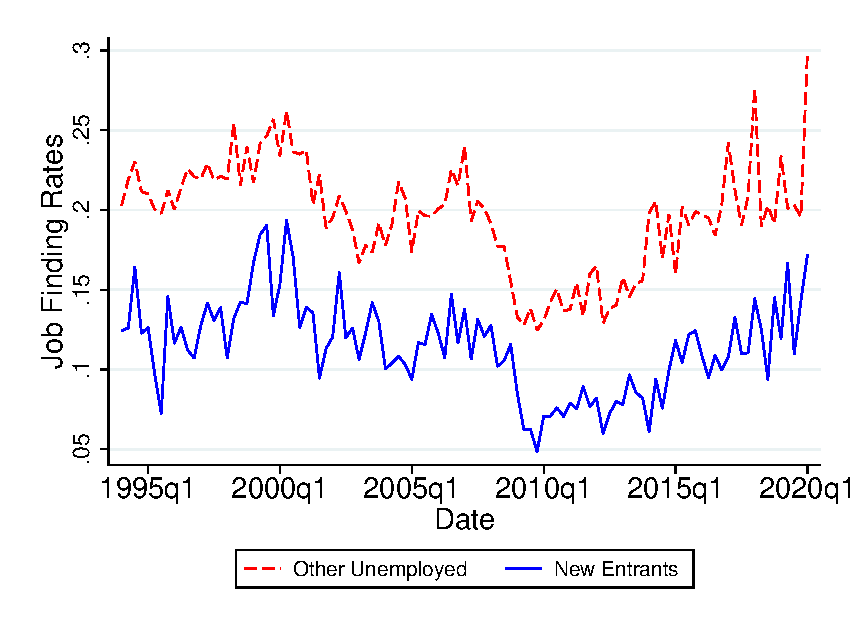
\includegraphics[width=0.85\textwidth]{JFR_16_24.eps}
\caption{Job-finding rates for unemployed workers 16-24 years old. Calculations based on monthly data of the Current Population Survey for 1994 to 2020.}
	\label{figure jfr}
\end{figure}

Several elements of our model are relatively non-standard and combined together in a common framework for the first time. 
Therefore, it is important to provide justification for some of the model’s novel ingredients. 
In particular, we discuss the following assumptions: (i) biased matching based on \cite{blanchard1994ranking} and \cite{petrongolo2001looking}, (ii) firm-provided training, and (iii) persistent skill loss during workers' first unemployment spell. 
We comment on each one of them in order.

First, the rationale for biased matching in favor of experienced workers is straightforward.
As can be seen in Figure \ref{figure jfr}, the job-finding rates of entrants are much lower than the job-finding rates of the experienced unemployed workers between 16 and 24 years old.\footnote{The difference is almost the same for workers between 16 and 64 years old as well. However, almost 85\% of entrants is between 16 and 24, hence we present the data for this age group.} 
The generalization of the \cite{blanchard1994ranking} ranking by \cite{petrongolo2001looking} provides a natural and tractable way to deliver job-finding rates consistent with this fact. Moreover, there are numerous pieces of anecdotal evidence indicating that many firms do not even consider workers without previous experience.
For example, an analysis of almost four million job postings on Linked-In since late 2017 showed that 35\% of postings for entry-level positions asked for years of prior relevant work experience.\footnote{\scriptsize{\url{https://www.bbc.com/worklife/article/20210916-why-inexperienced-workers-cant-get-entry-level-jobs}}}

Second, a crucial feature of our framework is the assumption that firms need to devote resources to train entrant workers.
These resources capture the fact that the experienced workers have to take time away from production to teach the necessary traits to the entrants. 
Examples of these traits include the ability to work in teams, follow instructions, understand and complete a task, or how to network.
There is a plethora of recent empirical papers documenting the importance of firm-provided training in the labor market.
\cite{ma2022human}, in a cross-country study, document that firm-provided training is a key determinant of workers' human capital.
\cite{bertheau2023makes}, using linked survey-administrative data from Denmark, find that one-third of employers consider the time to train new recruits as a major obstacle.

Moreover, there is a literature that highlights the empirical relevance of the inefficiency identified in this paper, namely, the idea that firms underhire inexperienced workers, since they are not fully compensated for the social benefit of the training they provide \citep{becker2009human, acemoglu1998firms, acemoglu1999beyond}.
An important empirical finding in this line of work is that firms provide general training which is not fully offset by lower wages; see \cite{loewenstein1998dividing} and \cite{autor2001temporary}.
\cite{pallais2014inefficient} aptly surveys this literature and concludes that ``...neither the theoretical nor the empirical literature shows that firms recoup the full value of their training investments resulting in their providing the optimal level of training'' (p. 3568).

%comparison with training: Acemoglu (ref report); Arellano Bover firms; JOLE Lents Roys RED; shisham review; guido, herkenhoff, lise; rosen and moen
%same mechanism but complemented with skill loss which creates intertemporal trade off and accounts for a large part of welfare losses
%comparison with skill loss: pissarides, sargent, kospentaris, ortego-marti; worker ranking is endogenous, depends on training and firm decision, which creates the intertmeporal trade off. skill loss happens BECAUSE of training


Third, there is compelling empirical evidence documenting that skill loss during the early unemployment spells has persistent negative effects on a worker's career.
\cite{arellano2022effect} shows that early-career unemployment shocks have negative effects on measured cognitive skills several decades later. 
Similarly, \cite{dinerstein2022human}, using quasi-experimental variation in unemployment duration at the beginning of teachers' careers in Greece, document strong negative effects of the length of unemployment on teachers' performance measured by students' test scores.
More generally, there is a large empirical literature, summarized by \cite{wachter2020persistent}, that highlights the persistence of the effects of labor market conditions upon entry for young workers on multiple outcomes later in their careers.


In the model, we have assumed that the unemployment spells after the first one have no effect on a worker's productivity.
We have made this assumption for various reasons. 
First, the consequences of unemployment for the skills of experienced workers is well-studied elsewhere and its inclusion would only make the model unnecessarily complicated.\footnote{For references on skill loss in unemployment, see \cite{pissarides1992loss}, \cite{ljungqvist1998european}, \cite{coles2000retraining}, \cite{ortego2016unemployment}, \cite{flemming2020skill}, and \cite{kospentaris2021unobserved}, among many others.}
More importantly, there is evidence that skill loss may be of limited importance in older ages.
For instance, \cite{cohen2023skill} find no indication for a decline in skills over the unemployment spell in the overall population in Germany and for the older workers in the US. In the authors' own words, ``This suggests that the negative consequences of unemployment might be a more relevant concern \textit{at younger ages}'' (p. 5, emphasis added).

%footnote material: Hensvik et al (2023) on the importance of connections for entrants: “We measure social contacts acquired during paid work during high school, and we rely on interacted classe-establishment fixed-effects models to isolate the effects of interest. One third of post-graduation matches are formed at establishments where youths worked during their studies. Graduates are much more likely to match with sites to which adult co-workers from these jobs have relocated. The importance of these job-finding channels is strongly counter-cyclical for young labour market entrants. Forsythe (2021) shows that firms hire disproportionally less young workers in recessions (what she calls cyclically selective hiring).

% Why not model with directed search only: i) presupposes too much market segmentation, in reality workers of different types do congest each other, ii) internships and government subisdies to training would be useless in a directed search world but we do see them in reality, hence real world must have some random search


\section{Analysis of the Model}\label{section analysis}

\subsection{Beveridge curves}\label{section beveridge}
Having described the economic environment, we are ready to proceed with the analysis of the model, starting with the derivation of the Beveridge curves. For this task, it is useful to inspect Figure \ref{figure model}, which illustrates the worker flows in and out of every state. While at first glance the figure may look complicated (workers could be in one of eight possible states), the logic is simple. 
\begin{figure}[!tb]
	\centering
	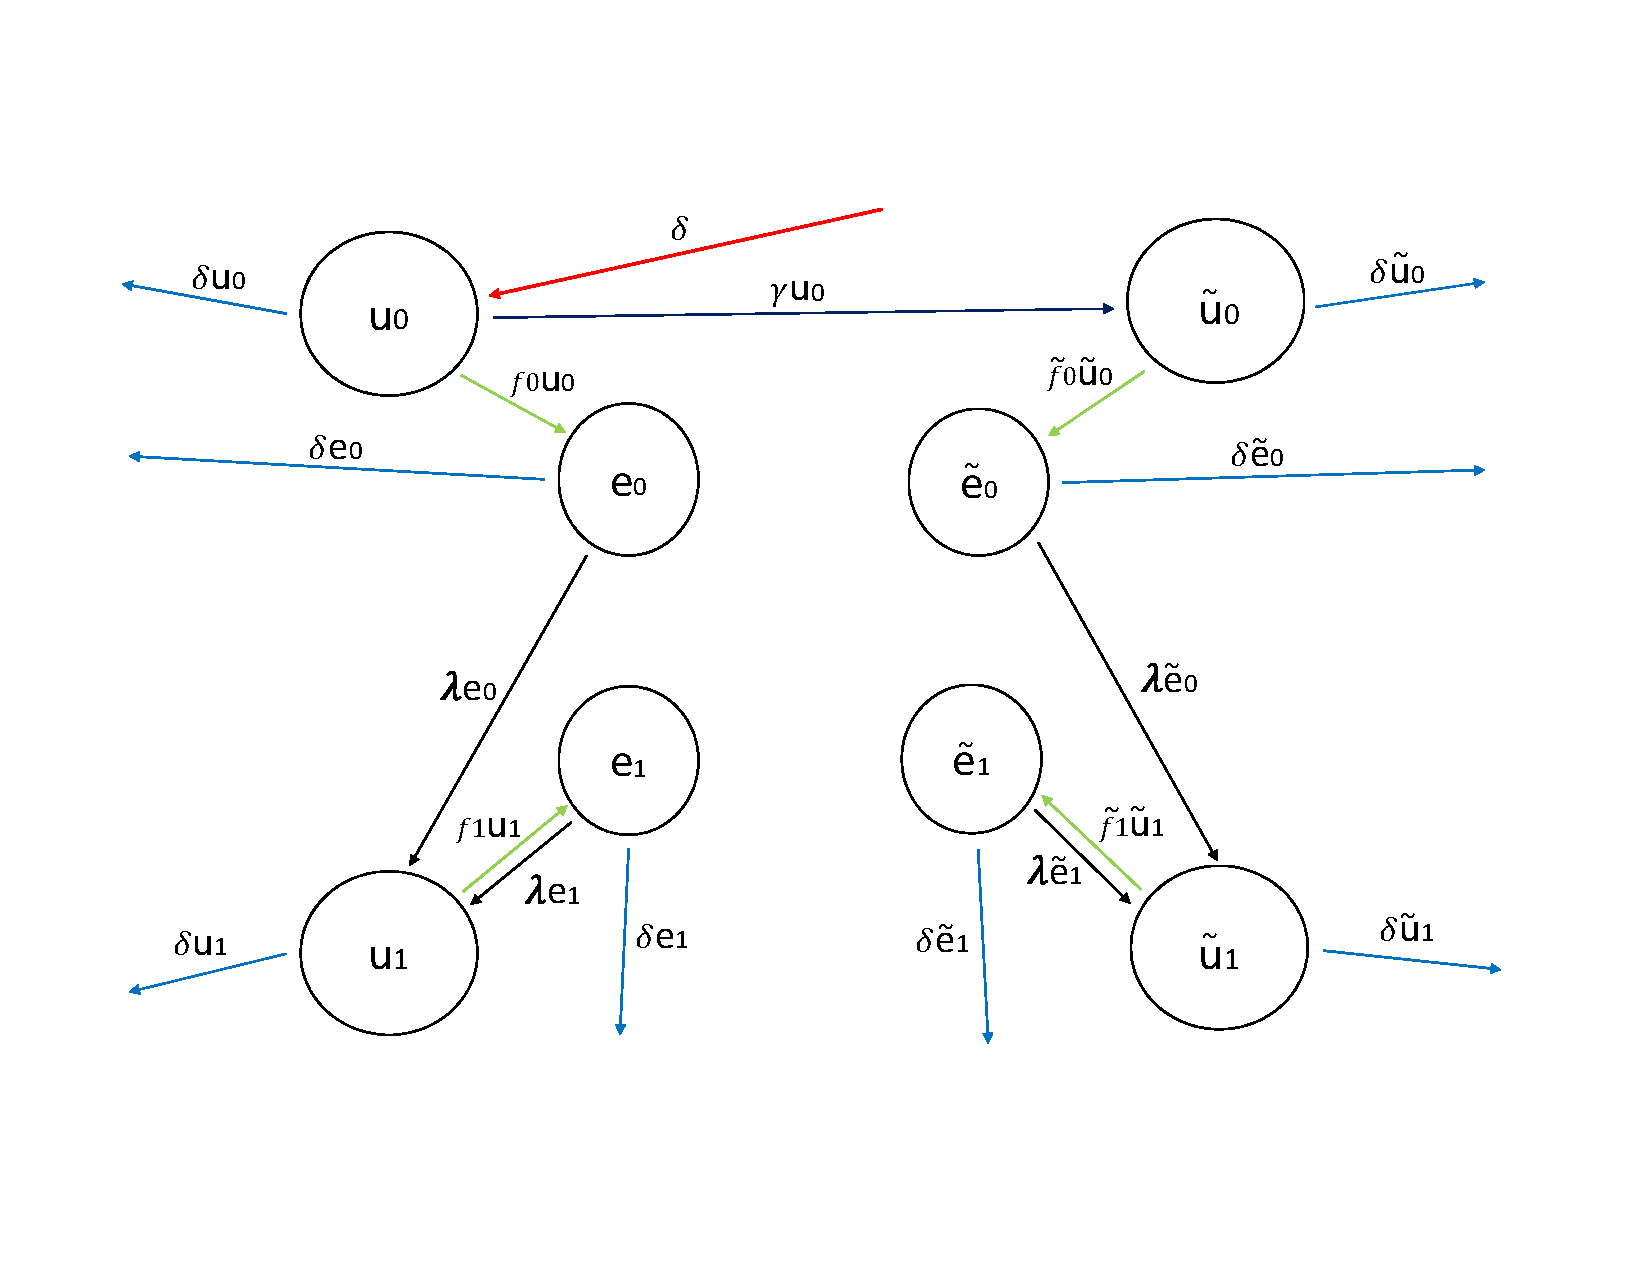
\includegraphics[width=1.05\linewidth]{empl_states.pdf}
	\vspace{0em}
	\caption{Worker flows in and out of the various states.}
	\label{figure model}
\end{figure}
New entrants come into the labor market as type-0 unemployed workers at rate $\delta$; this is indicated by the red arrow at the top of the graph. Then, at any state of the world, workers could get hit by the retirement shock and exit the labor market; these are the light blue arrows pointing away from the eight ``bubbles" representing the various states. There are also four black arrows starting from employment and pointing to unemployment bubbles; clearly, these are flows initiated by the job destruction shock. Notice that job destruction always leads to the bubble of ``experienced unemployed", which may be scarred ($\tilde{u_1}$) or not scarred ($u_1$). Green arrows indicate workers who found a job and are moving from unemployment to employment. As discussed, the rate at which this transition takes place is different for each worker type and governed by the \cite{petrongolo2001looking} matching process. Finally, the dark blue arrow starting at $u_0$ and pointing to $\tilde{u_0}$ captures the crucial group of workers who stayed in the ``inexperienced unemployed" pool for too long and got hit by the skill loss shock.  

Equating the flows in and out of each state, and after some algebra, we can show that the steady state measure of workers in the various states are as follows:  
\begin{eqnarray*}
u_0 &=& \frac{\delta}{\delta+\gamma+f_0},  \\
\tilde{u_0} &=& \frac{\gamma}{\delta+\Tilde{f_0}} \cdot  \frac{\delta}{\delta+\gamma+f_0},   \\
e_0 &=& \frac{f_0}{\delta+\lambda} \cdot \frac{\delta}{\delta+\gamma+f_0}, \\
\Tilde{e_0} &=& \frac{\Tilde{f_0}}{\delta+\lambda} \cdot \frac{\gamma}{\delta + \Tilde{f_0}} \cdot \frac{\delta}{\delta+\gamma+f_0},  \\
 u_1 &=& \frac{\lambda f_0}{(\gamma+\delta+f_0)(\delta+\lambda+f_1)},  \\
 e_1 &=& \frac{f_1}{\delta+\lambda} \cdot \frac{\lambda f_0}{(\gamma+\delta+f_0)(\delta+\lambda+f_1)}, \\
 \Tilde{u_1} &=& \frac{\lambda \gamma \Tilde{f_0}}{(\delta+\Tilde{f_0})(\gamma+\delta+f_0)(\delta+\lambda+\Tilde{f_1})}, \\
 \Tilde{e_1} &=& \frac{\Tilde{f_1}\lambda \gamma \Tilde{f_0}}{(\delta+\lambda)(\delta+\Tilde{f_0})(\gamma+\delta+f_0)(\delta+\lambda+\Tilde{f_1})}. 
\end{eqnarray*}


\subsection{Value Functions}\label{section value functions}
We move to the steady state value functions, and we start with the firms. We will let $q$ denote the arrival rate of workers to firms, and we will follow the usual notation, e.g, $\Tilde{q_0}$ will stand for the arrival rate of an inexperienced worker who has suffered skill loss. The various $q$'s are derived in Appendix \ref{section appendix proofs}. The value function of a vacant firm is given by 
\begin{equation}
   rV = -c + q_0 (J_0-V) + \Tilde{q_0}(\Tilde{J_0}-V) + q_1 (J_1-V) + \Tilde{q_1}(\Tilde{J_1}-V).\nonumber 
\end{equation}Of course, free entry implies that in equilibrium we must have $V=0$, therefore, we can state the free entry condition as 
\begin{equation}
   c= q_0 J_0 + \Tilde{q_0}\Tilde{J_0} + q_1 J_1 + \Tilde{q_1}\Tilde{J_1}.\label{eq free entry} 
\end{equation}

We also have four value functions for productive firms in the various states, i.e., for firms who matched with the four different types of workers (type 0, $\tilde{0}$, 1, and $\tilde{1}$). These are given as follows:   
\begin{eqnarray}
    rJ_0 &=&p-\kappa-w_0-\lambda J_0 - \delta J_0,\label{eq J0} \\
    r\Tilde{J_0} &=&p-\kappa-\Tilde{\kappa}-\Tilde{w_0}-\lambda \Tilde{J_0} - \delta \Tilde{J_0},\label{eq J0 tilde}\\
    rJ_1 &=&p-w_1-\lambda J_1 - \delta J_1, \label{eq J1} \\
        r\Tilde{J_1} &=&p-\Tilde{\kappa}-\Tilde{w_1}-\lambda \Tilde{J_1} - \delta \Tilde{J_1} . \label{eq J1 tilde}
    \end{eqnarray}

Next, consider the value functions of workers in the various states. Let $U$ ($W$) denote the value function of an unemployed (employed) worker. The remaining notation is standard. (For example, $\Tilde{W_1}$ is the value function of a worker who is employed, has had some work experience, but was hit by the skill loss shock during her youth.) The value functions for unemployed workers in the various states are given by: 
\begin{eqnarray}
    rU_0 &=& z+f_0(W_0-U_0)+\gamma(\Tilde{U_0}-U_0) - \delta U_0, \label{eq U0} \\
    r\Tilde{U_0} &=& z+\Tilde{f_0}(\Tilde{W_0}-\Tilde{U_0})- \delta \Tilde{U_0}, \label{eq U0 tilde}\\
    rU_1 &=& z+f_1(W_1-U_1)- \delta U_1, \label{eq U1}\\
    r\Tilde{U_1} &=& z+\Tilde{f_1}(\Tilde{W_1}-\Tilde{U_1})- \delta \Tilde{U_1}. \label{eq U1 tilde} 
\end{eqnarray}
The value functions for employed workers in the various states are given by: 
\begin{eqnarray}
    rW_0 &=&w_0+\lambda(U_1-W_0)- \delta W_0, \label{eq W0} \\
     r\Tilde{W_0} &=& \Tilde{w_0}+\lambda(\Tilde{U_1}-\Tilde{W_0})- \delta \Tilde{W_0}, \label{eq W0 tilde} \\
     rW_1 &=& w_1+\lambda(U_1-W_1)- \delta W_1, \label{eq W1} \\
     r\Tilde{W_1} &=& \Tilde{w_1}+\lambda(\Tilde{U_1}-\Tilde{W_1})- \delta \Tilde{W_1}. \label{eq W1 tilde}
     \end{eqnarray}
Notice that inexperienced workers who lose their first job now move to the pool of experienced unemployed workers. (That is precisely why the terms $U_1$ and $\Tilde{U_1}$ appear on the right-hand side of equations (\ref{eq W0}) and (\ref{eq W0 tilde})).  

Having described the value functions of all economic agents in detail, we are now ready to study the bargaining problems in the various types of meetings. 


\subsection{Bargaining problems}\label{section bargaining} 

\textbf{Bargaining in a type-1 meeting}

\medskip 

\noindent We begin with the description of the terms of trade in a meeting between a firm and an unemployed worker of type-1, which, as we shall see, is the simplest case. Solving the standard Nash bargaining problem implies that the following condition must be satisfied:
\begin{equation}
(1-\eta)(W_1-U_1) = \eta J_1. \label{eq bargain 1}
\end{equation}
This condition simply states that each party will enjoy a fraction of the total surplus of the match, and that fraction will be equal to her bargaining power. (Recall that $\eta$ is the bargaining power of the worker.) Replacing the value functions $W_1$ and $J_1$ from (\ref{eq W1}) and (\ref{eq J1}), respectively, allows us to write the wage of a type-1 worker as 
$$
w_1 = \eta p + (1-\eta)(r+\delta)U_1. 
$$Then, we can substitute $U_1$ from equation (\ref{eq U1}) into the last expression and write 
$$
w_1= \eta p + (1-\eta)z + (1-\eta)f_1(W_1-U_1)=  \eta p + (1-\eta)z + \eta f_1 J_1, 
$$where the second equality follows from (\ref{eq bargain 1}). Substituting $J_1$ one more time from equation (\ref{eq J1}), and solving for $w_1$, delivers the final version of our ``wage curve" for type-1 workers:  
\begin{equation}
 w_1 = \frac{\eta p (r+\lambda+\delta+f_1)+(1-\eta)z(r+\lambda+\delta)}{r+\lambda+\delta + \eta f_1}. \label{eq WC 1}
\end{equation}Clearly, this is a relationship between the wage for type-1 workers and their job arrival rate, which, in turn, depends on firm entry and market tightness. 

\bigskip 


\noindent \textbf{Bargaining in a type-$\Tilde{1}$ meeting}

\medskip 

\noindent Next, consider the bargaining problem between a firm and a worker who is experienced but suffered skill loss during her youth. Once again, we must have:
\begin{equation}
    (1-\eta)(\Tilde{W_1}-\Tilde{U_1}) = \eta \Tilde{J_1}. \nonumber  
\end{equation}As in the case of type-1 workers, we can replace the functions $\tilde{W_1}$ and $\tilde{J_1}$ from (\ref{eq W1 tilde}) and (\ref{eq J1 tilde}) into the last expression. Following identical steps, and after some algebra, one can easily derive the wage curve for type-$\tilde{1}$ workers: 
\begin{equation}
\Tilde{w_1} = \frac{\eta (p-\Tilde{\kappa}) (r+\lambda+\delta+\Tilde{f_1})+(1-\eta)z(r+\lambda+\delta)}{r+\lambda+\delta + \eta \Tilde{f_1}}. \label{eq WC1 tilde}
\end{equation}Once again, we obtain a relationship between the wage for type-$\tilde{1}$ workers and their job arrival rate, which, in turn, depends on firm entry and market tightness. 


\bigskip


\noindent \textbf{Bargaining in type-$\Tilde{0}$ meeting}

\medskip 

\noindent We now move to the bargaining problem between a firm and an inexperienced worker who suffered skill loss. In this case the surplus sharing rule is given by 
\begin{equation}
       (1-\eta)(\Tilde{W_0}-\Tilde{U_0}) = \eta \Tilde{J_0}.  \nonumber 
       \end{equation}As is standard, we first replace the value functions $\tilde{W_0}$ and $\tilde{J_0}$ from (\ref{eq W0 tilde}) and (\ref{eq J0 tilde}), respectively, which allows us to write the wage of a type-$\tilde{0}$ worker as
\begin{equation}
    \Tilde{w_0} = \eta (p-\kappa-\Tilde{\kappa})  - \lambda (1-\eta)(\Tilde{U_1} - \Tilde{U_0}) + (1-\eta)(r+\delta) \Tilde{U_0}. \label{eq w0 tilde first step}
    \end{equation}
    
Unlike the previous cases, where the wage depended on the value function of unemployment for that specific type (only), here $\Tilde{w_0}$ depends on both $\Tilde{U_0}$ {and} $\Tilde{U_1}$, and specifically on their difference $\Tilde{U_1}-\Tilde{U_0}$. To deal with this, subtract (\ref{eq U0 tilde}) from (\ref{eq U1 tilde}) to obtain 
\begin{equation}
\Tilde{U_1}-\Tilde{U_0} = \frac{\Tilde{f_1}(\Tilde{W_1}-\Tilde{U_1}) - \Tilde{f_0}(\Tilde{W_0}-\Tilde{U_0})}{r+\delta}.\label{eq U1 tilde-U0 tilde}
    \end{equation}To obtain a useful expression for the term $\Tilde{W_1}-\Tilde{U_1}$, that now appears in (\ref{eq U1 tilde-U0 tilde}), subtract (\ref{eq U1 tilde}) from (\ref{eq W1 tilde}), to get  
\begin{equation}
\Tilde{W_1}-\Tilde{U_1} = \frac{\Tilde{w_1}-z}{r+\delta+\lambda+\Tilde{f_1}}. \label{eq W1tilde - U1 tilde}
\end{equation} Substitute equation (\ref{eq W1tilde - U1 tilde}) into (\ref{eq U1 tilde-U0 tilde}), and the resulting outcome into equation (\ref{eq w0 tilde first step}), and, after some some algebra, one can arrive at the wage curve for the type-$\Tilde{0}$ worker, specifically: 
\begin{equation} 
\begin{split}
\Tilde{w_0} = \frac{1}{r+\delta+\eta \Tilde{f_0}}\big[\eta(p-\kappa-\Tilde{\kappa})(r+\delta+ \Tilde{f_0}) &+ \\
+\frac{(r+\delta+\lambda)(r+\delta+\Tilde{f_1})}{r+\delta+\lambda+\Tilde{f_1}}(1-\eta)z &- \frac{\lambda(1-\eta)\Tilde{f_1}}{r+\delta+\lambda+\Tilde{f_1}}\Tilde{w_1} \big]. \label{eq WC0 tilde}
\end{split}
\end{equation}

Inspection of the last wage curve reveals that, in this case, the wage for type-$\tilde{0}$ workers is not only a function of this type's job arrival rate (as was the case for type-1 and type-$\tilde{1}$ workers). The wage $\Tilde{w_0}$ also depends on the wage that type-$\tilde{1}$ workers make. The intuition is clear. When a type-$\tilde{0}$ worker meets a firm, working for that firm is the step that will allow her to move out of the ``inexperienced" state, and earn the wage $\Tilde{w_1}$ for the rest of her life. This is precisely, why the term $\Tilde{w_1}$ enters equation (\ref{eq WC0 tilde}) with a minus: a higher (future) wage $\Tilde{w_1}$ induces the type-$\tilde{0}$ worker to be more eager to accept a lower (current) wage $\Tilde{w_0}$, since that lower wage comes together with the opportunity of abandoning the bad ``inexperienced'' stage once and for all. 

\bigskip 
    
\noindent \textbf{Bargaining in type-0 meeting}

\medskip 

\noindent The last type of meeting is the one between a firm and an unskilled worker who has not yet been hit by the skill loss shock. The surplus sharing rule is given by 
\begin{equation}
       (1-\eta)(W_0-U_0) = \eta J_0 .  \nonumber 
\end{equation}Following standard steps, substitute ${W_0}$ and ${J_0}$ from (\ref{eq W0}) and (\ref{eq J0}), respectively, to write the wage of a type-0 worker as
\begin{equation}
    w_0 = \eta(p-\kappa) - (1-\eta)\lambda(U_1 - U_0) + (1-\eta)(r+\delta) U_0. \nonumber 
    \end{equation}
    
Just like in the case of type-$\tilde{0}$ workers (and unlike the cases of type-1 and type-$\tilde{1}$ workers), the wage for the types under consideration (also) depends on the differential term ${U_1}-{U_0}$. Since the steps for deriving the final version of the wage curve are virtually identical to the case of type-$\tilde{0}$ workers presented above, we will skip the details and move directly to the final formula:  
\begin{equation}\label{eq WC0}
 \begin{split}
         w_0 & = \frac{r+\delta+\gamma +f_0}{r+\delta+\gamma+\eta f_0}\eta (p-\kappa) + \frac{(r+\lambda+\delta)(r+f_1+\delta)(r+\gamma+\delta)}{(r+\delta)(r+\delta+\gamma + \eta f_0)(r+\delta+\lambda+f_1)} (1-\eta) z + \\  
 & + \frac{\gamma \Tilde{f_0}\eta(p-\kappa-\Tilde{\kappa}-\Tilde{w_0})}{(r+\delta)(r+\delta+\gamma + \eta f_0)} - \frac{(1-\eta)\lambda f_1 (r+\gamma+\delta)w_1}{(r+\delta)(r+\delta+\gamma + \eta f_0)(r+\delta+\lambda+f_1)}. 
    \end{split}
\end{equation}

The wage curve for type-0 workers admits an interpretation that is similar to the one following the wage curve for type-$\tilde{0}$ workers, i.e., equation (\ref{eq WC0 tilde}). The wage that type-0 workers are willing to accept is not just a function of their job arrival rate: ${w_0}$ also depends on ${w_1}$ \textit{and} $\tilde{w_0}$. Why ${w_0}$ depends on ${w_1}$ should now be obvious, given our earlier discussion: the type-0 worker realizes that if she agrees to work for that firm, she will be able to move out of the inexperienced state and earn the wage ${w_1}$ henceforth. Why does ${w_0}$ also depend on $\tilde{w_0}$? When the type-0 worker agrees to work for the firm with which she has matched, she realizes that she will never again be subject to the skill loss shock. Thus, what the worker \textit{would} have made if she turned down the firm's offer and continued searching (and being subject to the skill loss shock), i.e., the wage $\tilde{w_0}$, enters the currently negotiated wage through her outside option.   


\subsection{Definition of Steady State Equilibrium}\label{section definition of equil} 

We conclude this section with a formal definition of equilibrium. 

\begin{definition}\label{definition equilibrium}
    A steady state equilibrium in our model is a list of wages for the four types of workers $(w_0, \Tilde{w_0}, w_1, \Tilde{w_1})$, a measure of vacant firms $v$, and measures of unemployed and employed workers in the various states $(u_0, \Tilde{u_0}, u_1, \Tilde{u_1}, e_0, \Tilde{e_0}, e_1, \Tilde{e_1})$, satisfying the free entry condition (\ref{eq free entry}), the four wage curves (\ref{eq WC 1}), (\ref{eq WC1 tilde}), (\ref{eq WC0 tilde}), and (\ref{eq WC0}), and the eight Beveridge curves reported at the end of Section \ref{section beveridge}.\footnote{\,Implicit in this definition are the queue lengths $(b_0,\tilde{b_0},b_1,\tilde{b_1})$, defined in equation (\ref{eq queue lengths}) as functions of the various unemployment measures and $v$. In turn, these queue lengths are used to determine the various job-finding rates $(f_0,\tilde{f_0},f_1,\tilde{f_1})$, which appear in the Beveridge curves, as well as the firms' worker-finding rates $(q_0,\tilde{q_0},q_1,\tilde{q_1})$ (described in Appendix \ref{section appendix proofs}), which appear in the job creation curve.}   
\end{definition} 



%---------------------------------------------------------------------------------


\section{Government Interventions}\label{section policy interventions}

The discussion so far reveals that our model is characterized by a prominent market failure. Firms who hire entrant workers provide a \textit{public good} to society by transforming them into experienced and, hence, (more) productive workers. However, the firms cannot internalize the societal benefits of this public service, and they rationally choose to discriminate against inexperienced workers. This bias increases the inexperienced workers' unemployment duration, which, in turn, raises their exposure to skill loss, a skill loss which permanently scars the workers, thus affecting their productivity when they are hired by other firms later in their lifetime.

  
It is obvious that in this environment there is scope for government intervention. Since the root of the inefficiency lies in the firms' decision to underhire inexperienced workers (see also \cite{pallais2014inefficient} and the references therein), we consider three possible government interventions whose common goal is to alleviate the bias against this group of workers, reduce their exposure to the skill loss shock and, hopefully, increase welfare. We start with a short description of the idea behind each of these three interventions, and then we analyze them in detail in the rest of this section. A \textit{vis-\`a-vis} comparison of the effectiveness of each intervention will follow in Section \ref{section results}. 

\medskip

\underline{\textit{Intervention 1: ``Unbiased matching".}} We dub the first intervention ``unbiased matching", as it describes the case where the government makes it \textit{illegal} for firms to discriminate against any group of workers. Even though one could argue that this intervention is somewhat unrealistic (firms have the right to not hire less productive workers), it is still interesting, from a theoretical point of view, to study a benchmark model without biased matching, which has been a staple of the analysis so far, and appears to be the root of the ongoing inefficiency. Comparing the baseline model with the economy under Intervention 1 can tell us how much welfare can improve if the firms' bias against inexperienced workers was eradicated. In technical terms, the unbiased matching version of the model simply replaces the \cite{petrongolo2001looking} matching process with a standard \cite{pissarides2000equilibrium} matching function where all workers meet firms at the same rate. 

\medskip

\underline{\textit{Intervention 2: ``Government subsidies".}} Our second intervention is one where the government raises funds to subsidize firms who hire less productive workers. Subsidies are designed so that firms are effectively \textit{indifferent} among the various types of workers, so that they \textit{choose} to not discriminate against any type of workers. Thus, one can think of Intervention 2 as a market-based way of achieving what Intervention 1 achieves by law, i.e., unbiased matching.\footnote{\,Despite this similarity, the two versions of the model do not lead to the same equilibrium outcomes, and the two interventions are not equally effective at improving welfare. For details see Section \ref{section results}.} 

\medskip

\underline{\textit{Intervention 3: ``Internships".}} The third intervention explores the possibility that the wage of entrant/inexperienced workers is not determined endogenously in the model, but chosen exogenously by the government. We dub this intervention ``internships" because it assumes that inexperienced workers are not compensated based on their true productivity, but they are treated as trainees whose salary is predetermined and exogenous. We think this is a crucial element of an internship, although we realize that other important elements of real-world internships are absent from our model. In any case, the term ``internship" here is just a tag that will summarize Intervention 3. This intervention will allow firms to employ inexperienced workers at lower salaries, effectively lowering the bias against these workers and mitigating the inefficiency described in the beginning of this section.  



\subsection{Intervention 1: Unbiased matching}\label{section unbiased matching}

\textbf{Beveridge Curves} 

\noindent Consider first the Beveridge curves for this version of our model. When it is illegal for firms to discriminate against certain types of workers, all workers match with firms at the same rate. All the Beveridge curves reported at the end of Section \ref{section beveridge} are still valid, but the various matching rates are now equal. That is, $f_0=\Tilde{f_0}=f_1=\Tilde{f_1}=f$, where the common arrival rate $f$ is now given by a standard (unbiased) matching process, i.e., 
\begin{equation}
f=\frac{m(u,v)}{u},\label{eq definition of common f} 
\end{equation}with $u$ representing the total mass of unemployed workers (of all types). 


\bigskip 

\noindent \textbf{Value Functions}

\noindent Next, we move to the value functions under the regime of Intervention 1, starting with the firms. With unbiased matching, the probability that a firm meets a worker of a specific type depends only on that type's relative representation in the pool of unemployed. Letting $q$ denote the arrival rate of a(ny) worker to the typical firm, i.e., $q=m(u,v)/v$, the value function of a vacant firm is given by 
\begin{equation}
   rV = -c + q \left[\frac{u_0}{u}(J_0-V) + \frac{\Tilde{u_0}}{u}(\Tilde{J_0}-V) + \frac{u_1}{u}(J_1-V) +  \frac{\Tilde{u_1}}{u}(\Tilde{J_1}-V) \right].\nonumber 
\end{equation}As is standard, free entry implies that in equilibrium $V=0$, therefore, we can state the free entry condition as 
\begin{equation}
 c = \frac{q}{u} \left({u_0} J_0 + \Tilde{u_0} \Tilde{J_0} + {u_1} J_1 +  \Tilde{u_1} \Tilde{J_1} \right).\label{eq free entry intervention 1} 
\end{equation}

Even though the process through which firms meet workers is different compared to the baseline model of Section \ref{section analysis}, once a firm has met a specific type of worker, the value functions for productive firms in the various states remain the same, i.e., they are still given by equations (\ref{eq J0})-(\ref{eq J1 tilde}). 
%, which we repeat here for the reader's convenience. 
%\begin{eqnarray}
%rJ_0 &=&p-\kappa-w_0-\lambda J_0 - \delta J_0,\nonumber \\
%    r\Tilde{J_0} &=&p-\kappa-\Tilde{\kappa}-\Tilde{w_0}-\lambda \Tilde{J_0} - \delta \Tilde{J_0},\nonumber\\
%    rJ_1 &=&p-w_1-\lambda J_1 - \delta J_1, \nonumber  \\
%        r\Tilde{J_1} &=&p-\Tilde{\kappa}-\Tilde{w_1}-\lambda \Tilde{J_1} - \delta \Tilde{J_1} . \nonumber 
%\end{eqnarray}

Moving on to the workers, the value functions for unemployed workers in the various states are given by: 
\begin{eqnarray}
    rU_0 &=& z+f(W_0-U_0)+\gamma(\Tilde{U_0}-U_0) - \delta U_0, \label{eq U0 inter 1}  \\
    r\Tilde{U_0} &=& z+{f}(\Tilde{W_0}-\Tilde{U_0})- \delta \Tilde{U_0}, \label{eq U0 tilde inter 1}\\
    rU_1 &=& z+f(W_1-U_1)- \delta U_1, \label{eq U1 inter 1}\\
    r\Tilde{U_1} &=& z+{f}(\Tilde{W_1}-\Tilde{U_1})- \delta \Tilde{U_1}.\label{eq U1 tilde inter 1}
\end{eqnarray}Notice that these expressions are almost identical to the value functions (\ref{eq U0})-(\ref{eq U1 tilde}) reported in Section \ref{section value functions}, with the only difference being that the various arrival rates of that section have now been replaced by the common rate $f$, defined in equation (\ref{eq definition of common f}). 

The last set of value functions for this model specification concerns employed workers. Since employed workers have already matched with a firm, the different matching process assumed in this section will not affect their employment value functions, which are still given by equations (\ref{eq W0})-(\ref{eq W1 tilde}) in Section \ref{section value functions}. 
%, and we repeat here for convenience:  
%\begin{eqnarray*}
%    rW_0 &=&w_0+\lambda(U_1-W_0)- \delta W_0, \\
%     r\Tilde{W_0} &=& \Tilde{w_0}+\lambda(\Tilde{U_1}-\Tilde{W_0})- \delta \Tilde{W_0}, \\
%    rW_1 &=& w_1+\lambda(U_1-W_1)- \delta W_1, \\
%     r\Tilde{W_1} &=& \Tilde{w_1}+\lambda(\Tilde{U_1}-\Tilde{W_1})- \delta \Tilde{W_1}.
%     \end{eqnarray*}

\bigskip 

\noindent \textbf{Bargaining problems}

\noindent As the discussion so far reveals, the only parts of the analysis that are affected by the adoption of the new (unbiased) matching process are those that take place    \textit{before} a firm and a worker match. Consequently, all the derivations of the wage curves in Section \ref{section bargaining} remain valid, with the only difference being that the various arrival rates will now be replaced by the common arrival rate $f$. This observation also sheds some light on the economic insights of this intervention. The government, under Intervention 1, does not intervene in the labor market to change the way in which firms and workers produce or negotiate over the wages. It only intervenes by stating that discriminating against any type of worker, at the recruiting stage, is illegal. By doing this, the government ensures that \textit{all} types of workers have the same matching rate, which, in turn, ensures that entrant/inexperienced workers will not stay unemployed for a prolonged period of time, thus risking a skill loss that will scar them for the rest of their career. We will discuss the effectiveness of this intervention, and how it compares to the alternatives, in Section \ref{section results}. 

Given that the derivations of the wage curves in Section \ref{section bargaining} remain unaltered, we will not repeat them here, and we will only report the wage curves for the four types of workers, reminding the reader that they are identical to ones reported in equations (\ref{eq WC 1}), (\ref{eq WC1 tilde}), (\ref{eq WC0 tilde}), and (\ref{eq WC0}), once one has replaced the various $f$'s with the common arrival rate $f$ defined in equation (\ref{eq definition of common f}). More precisely, we have:    
\begin{equation}
 w_1 = \frac{\eta p (r+\delta+\lambda+f)+(1-\eta)z(r+\delta+\lambda)}{r+\delta+\lambda + \eta f},  \label{eq WC1 inter 1}
\end{equation}
\begin{equation}
\Tilde{w_1} = \frac{\eta (p-\Tilde{\kappa}) (r+\delta+\lambda+f)+(1-\eta)z(r+\delta+\lambda)}{r+\delta+\lambda + \eta f},  \label{eq WC1 tilde inter 1}
\end{equation}
\begin{equation} \label{eq WC0 tilde inter 1}
\hspace{-1cm}\Tilde{w_0}  = \frac{r+\delta+ f}{r+\delta+\eta {f}} 
\left[\eta(p-\kappa-\Tilde{\kappa}) +\frac{r+\delta+\lambda}{r+\delta+\lambda+f}(1-\eta)z - \frac{\lambda(1-\eta){f}}{(r+\delta+\lambda+f)(r+\delta+ f)}\Tilde{w_1} \right],
\end{equation}
\begin{equation} \label{eq WC0 inter 1}
\begin{split}
 w_0  & = \frac{r+\delta+\gamma +f}{r+\delta+\gamma+\eta f}\eta (p-\kappa) + \frac{(r+\delta+\lambda)(r+\delta+f)(r+\delta+\gamma)}{(r+\delta)(r+\delta+\gamma + \eta f)(r+\delta+\lambda+f)} (1-\eta) z  \\
 & + \frac{\gamma f \eta(p-\kappa-\Tilde{\kappa}-\Tilde{w_0})}{(r+\delta)(r+\delta+\gamma + \eta f)} - \frac{(1-\eta)\lambda f (r+\delta+\gamma)w_1}{(r+\delta)(r+\delta+\gamma + \eta f)(r+\delta+\lambda+f)}.
\end{split}
\end{equation}

%\begin{equation}
%    \begin{multlined}
 %        w_0 = \frac{r+\delta+\gamma +f}{r+\delta+\gamma+\eta f}\eta (p-\kappa) + \frac{(r+\lambda+\delta)(r+f+\delta)(r+\gamma+\delta)}{(r+\delta)(r+\delta+\gamma + \eta f)(r+\lambda+\delta+f)} (1-\eta) z \label{eq WC0 inter 1} \\  
% + \frac{\gamma {f}}{(r+\delta)(r+\delta+\gamma + \eta f)}\eta(p-\kappa-\Tilde{\kappa}-\Tilde{w_0}) - \frac{(1-\eta)\lambda f (r+\gamma+\delta)w_1}{(r+\delta)(r+\delta+\gamma + \eta f)(r+\lambda+\delta+f)}. \nonumber 
%    \end{multlined}
% \end{equation}

\bigskip 

\begin{definition}\label{definition equil inter 1}
    A steady state equilibrium, under Intervention 1, is a list of wages for the four types of workers $(w_0, \Tilde{w_0}, w_1, \Tilde{w_1})$, a measure of vacancies $v$, and measures of unemployed and employed workers in the various states $(u_0, \Tilde{u_0}, u_1, \Tilde{u_1}, e_0, \Tilde{e_0}, e_1, \Tilde{e_1})$, satisfying the free entry condition (\ref{eq free entry intervention 1}), the four wage curves (\ref{eq WC1 inter 1}), (\ref{eq WC1 tilde inter 1}), (\ref{eq WC0 tilde inter 1}), and (\ref{eq WC0 inter 1}), and eight Beveridge curves, which are the ones reported at the end of Section \ref{section beveridge}, after one replaces the various $f$'s with the common arrival rate $f$ defined in equation (\ref{eq definition of common f}).
\end{definition} 



\subsection{Intervention 2: Government subsidies}\label{section government subsidies}


Unlike Intervention 1, where the government could impose unbiased matching by law (i.e., firms were not allowed to discriminate against any worker type), here the government raises funds to subsidize firms who hire less productive workers. More specifically, each firm who hires a type-0 worker will receive a (flow) subsidy $\sigma_0$, each firm who hires a type-$\tilde{0}$ worker will receive a subsidy $\tilde{\sigma_0}$, and each firm who hires a type-$\tilde{1}$ worker will receive a subsidy $\tilde{\sigma_1 }$. To raise funding for these subsidies, every active firm pays a flat (lump-sum) tax equal to $\tau$. The aforementioned subsidies are designed so that firms are \textit{effectively indifferent} among the various types of workers. Thus, one can think of Intervention 2 as a market-based (as opposed to legislative) way of achieving unbiased matching. 


\bigskip 

\noindent \textbf{Beveridge Curves} 

\noindent Even though under Intervention 2 this happens for different reasons (subsidies rather than anti-discriminating laws), the end result is that firms are indifferent among the various types of workers. This simply means that all workers face identical job-finding rates, and, consequently, all the Beveridge curves remain the same as the ones described in Section \ref{section unbiased matching}. This, in turn, means that relevant Beveridge curves are the ones reported at the end of Section \ref{section beveridge}, but with $f_0=\Tilde{f_0}=f_1=\Tilde{f_1}=f$ (where $f$ was defined in equation (\ref{eq definition of common f})). 


\bigskip 

\noindent \textbf{Value Functions}

\noindent Next, we move to the value functions under the regime of Intervention 2, starting with the firms. Using our standard notation, the value functions of firms who have matched with the various types of workers are given by
\begin{eqnarray}
    rJ_0 &=&p-\kappa - w_0 + \sigma_0 - \tau -\lambda J_0 - \delta J_0,\label{eq J0 inter 2} \\
    r\Tilde{J_0} &=& p-\kappa-\Tilde{\kappa}-\Tilde{w_0}+ \Tilde{\sigma_0} - \tau - \lambda \Tilde{J_0} - \delta \Tilde{J_0},\label{eq J0 tilde inter 2}\\
    rJ_1 &=&p-\tau-w_1-\lambda J_1 - \delta J_1, \label{eq J1 inter 2} \\
    r\Tilde{J_1} &=&p-\Tilde{\kappa}-\Tilde{w_1}+ \Tilde{\sigma_1} - \tau-\lambda \Tilde{J_1} - \delta \Tilde{J_1}. \label{eq J1 tilde inter 2}
    \end{eqnarray}
However, recall that here the various subsidies are designed to make firms indifferent among the various types of workers. This implies that $J_0=\Tilde{J_0}=J_1=\Tilde{J_1}=J$. This greatly simplifies the value function of a vacant firm, which is now given by 
\begin{equation}
   rV = -c + q (J-V), \nonumber 
\end{equation}where, as before, $q=m(u,v)/v$, is the worker-finding rate of the typical firm. Free entry implies that in equilibrium we must have  
\begin{equation}
 c = q J.\label{eq free entry intervention 2} 
\end{equation}

Since all types of workers under Intervention 2 have identical job-finding rates (albeit for different reasons), the value functions for unemployed workers reported in Section \ref{section unbiased matching}, i.e., equations (\ref{eq U0 inter 1})-(\ref{eq U1 tilde inter 1}), remain valid. 
%We repeat them here for the reader's convenience. 
%\begin{eqnarray*}
%    rU_0 &=& z+f(W_0-U_0)+\gamma(\Tilde{U_0}-U_0) - \delta U_0, \\
%    r\Tilde{U_0} &=& z+{f}(\Tilde{W_0}-\Tilde{U_0})- \delta \Tilde{U_0}, \\
%    rU_1 &=& z+f(W_1-U_1)- \delta U_1, \\
%    r\Tilde{U_1} &=& z+{f}(\Tilde{W_1}-\Tilde{U_1})- \delta \Tilde{U_1}.
%\end{eqnarray*}
The value functions for employed workers are also identical to the ones reported in Section \ref{section unbiased matching}, which, in turn, are identical to the value functions given by equations (\ref{eq W0})-(\ref{eq W1 tilde}) in Section \ref{section value functions}. 
%We simply repeat them here for convenience:  
%\begin{eqnarray*}
%    rW_0 &=&w_0+\lambda(U_1-W_0)- \delta W_0, \\
%     r\Tilde{W_0} &=& \Tilde{w_0}+\lambda(\Tilde{U_1}-\Tilde{W_0})- \delta \Tilde{W_0}, \\
%     rW_1 &=& w_1+\lambda(U_1-W_1)- \delta W_1, \\
%     r\Tilde{W_1} &=& \Tilde{w_1}+\lambda(\Tilde{U_1}-\Tilde{W_1})- \delta \Tilde{W_1}.
%     \end{eqnarray*}

Before we move to the bargaining problems, we present an auxiliary result that will significantly simplify our task.

\begin{lemma}\label{lemma all ws the same}
Under Intervention 2, all types of workers must receive the same wage, i.e., $w_0=\Tilde{w_0}=w_1=\Tilde{w_1}=w$.     \end{lemma}
\begin{proof}
See Appendix \ref{section appendix proofs}.
\end{proof}

The proof of the lemma has been relegated to the appendix, but the statement is quite intuitive. Since the government's intervention makes firms indifferent among the various types of workers, it turns out that all the workers will make the same wage in equilibrium. It should also be obvious why Lemma \ref{lemma all ws the same} simplifies the analysis: under Intervention 2, we will only have to solve one bargaining problem, instead of four. 

\bigskip 

\noindent \textbf{Bargaining problem(s)}

Since the various $J_i$ terms are all equal to each other, and since the bargaining problem in each type of meeting would imply $(1-\eta)(W_i-U_i)=\eta J_i$, we must have that the various $W_i-U_i$ terms are also equal to each other. Thus, instead of solving four distinct bargaining problems, in this specification of the model we only need to solve one bargaining problem. As one can see in detail in the proof of Lemma \ref{lemma all ws the same}, the various $W_i-U_i$ terms are all equal to 
$$
W-U= \frac{w-z}{r+\lambda+\delta+f},   
$$where $w$ is the common wage established in Lemma \ref{lemma all ws the same}. As for the $J$ term, we can simply replace it from the free entry condition, i.e., equation (\ref{eq free entry intervention 2}). Then, the standard bargaining protocol, prescribing that $(1-\eta)(W-U)=\eta J$, here implies that
%$$(1-\eta)\frac{w-z}{r+\lambda+\delta+f} = \eta \, %\frac{c}{q},$$or, equivalently, 
\begin{equation}
w = z + \frac{\eta}{1-\eta} \, \frac{c(r+\delta+\lambda+f)}{q}, \label{eq wage curve inter 2} 
\end{equation}which is our (unique) wage curve under Intervention 2. 


\bigskip 

\noindent \textbf{The size of the tax and the various subsidies}

\noindent Before we proceed to the definition of equilibrium under Intervention 2, we must characterize the size of the various subsidies and the flat tax. Exploiting equations (\ref{eq J0 inter 2})-(\ref{eq J1 tilde inter 2}), and keeping in mind that $J_0=\Tilde{J_0}=J_1=\Tilde{J_1}=J$, we can deduce that 
$$p-\kappa-w_0-\tau+\sigma_0 = p-\kappa-\Tilde{\kappa}-\Tilde{w_0}-\tau+\Tilde{\sigma_0}=p-\tau-w_1=p-\Tilde{\kappa}-\tau-\Tilde{w_1}+\Tilde{\sigma_1}.$$
But since Lemma \ref{lemma all ws the same} has established that all the wages must be equal (and since all firms pay the same flat tax $\tau$), we have 
\begin{eqnarray}
    \sigma_0&=&\kappa,\label{eq subsidy 0} \\
    \Tilde{\sigma_0}&=&\kappa + \Tilde{\kappa},\label{eq subsidy 0 tilde}\\
    \Tilde{\sigma_1}&=&\Tilde{\kappa}.\label{eq subsidy 1 tilde} 
\end{eqnarray}Again, this is intuitive. The only way in which the government can make firms indifferent among the various types of workers is by fully covering the ``cost" associated with hiring a less productive type (i.e., anyone other than type-1). 
%For a type-0 worker that cost is the training cost $\kappa$. For a type-$\tilde{1}$ worker the government should cover the term $\tilde{\kappa}$, which captures the reduced productivity of a worker who suffered skill loss during her youth. Lastly, for a type-$\tilde{0}$ worker the government should subsidize both $\kappa$ and $\tilde{\kappa}$ to induce the firm to hire this rather unproductive worker (at the same rate as other workers). 

The last item we need to specify is the flat tax rate.  %Letting the various $e$ terms denote the measures of employed workers in the various states (defined in detail at the end of Section \ref{section beveridge})
A balanced government budget constraint means that $e \cdot \tau = e_0 \sigma_0 + \Tilde{e_0}\Tilde{\sigma_0} + \Tilde{e_1}\Tilde{\sigma_1}$, which implies that\footnote{\,The term $e$ is the total measure of employed workers, that is, $e= e_0+ \Tilde{e_0}+e_1+\tilde{e_1}$.} 
\begin{equation}
    \tau = \frac{\kappa e_0 + (\kappa + \Tilde{\kappa})\, \Tilde{e_0} + \Tilde{\kappa}\Tilde{e_1}}{e}. \label{eq tau}
\end{equation}



\medskip 

\begin{definition}\label{definition equil inter 2}
    A steady state equilibrium, under Intervention 2, is a (common) wage, $w$, for all types of workers, a list of subsidies $(\sigma_0, \Tilde{\sigma_0}, \Tilde{\sigma_1})$, a flat tax, $\tau$, paid by all active firms, a measure of vacancies $v$, and measures of unemployed and employed workers in the various states $(u_0, \Tilde{u_0}, u_1, \Tilde{u_1}, e_0, \Tilde{e_0}, e_1, \Tilde{e_1})$. The three types of subsidies satisfy equations (\ref{eq subsidy 0}), (\ref{eq subsidy 0 tilde}), and (\ref{eq subsidy 1 tilde}), respectively, and the tax satisfies equation (\ref{eq tau}). The remaining equilibrium variables satisfy the free entry condition (\ref{eq free entry intervention 2}), the wage curve (\ref{eq wage curve inter 2}), and eight Beveridge curves, which are the ones reported at the end of Section \ref{section beveridge}, after one replaces the various $f$'s with the common arrival rate $f$ defined in equation (\ref{eq definition of common f}). 
    \end{definition} 


\subsection{Intervention 3: Internships} \label{section internships}

Our third and last intervention is the one dubbed ``internships". Here, we explore the possibility that the wage of entrant/inexperienced workers is not determined endogenously in the model (i.e., by Nash bargaining), but it is chosen exogenously by the government. Let us denote the wages of type-0 and type-$\Tilde{0}$ workers by $w_0$ and $\Tilde{w_0}$, respectively. For now, we treat them as exogenous parameters, but in Section \ref{section results} we will discuss how changes in these two terms affect equilibrium welfare. All experienced workers (of type-1 and type-$\Tilde{1}$) will continue to make wages that are determined by Nash bargaining. 

A natural question that arises is whether firms still have an incentive to discriminate against certain types of workers. Think, for example, of type-0 workers. These workers must be trained by the firms (their productivity is $p-\kappa$), but their wage is given exogenously by $w_0$, which could be very low (perhaps even zero). Whether firms would prefer to hire a type-1 to a type-0 worker depends on the size of $\kappa$ and $w_0$. In fact, as long as $\kappa$ is not too large, the government could always choose $w_0$ to be low enough, so that firms prefer to match with a type-0 worker and discriminate against type-1 workers. Since, for now, we have decided to treat $w_0$ and $\Tilde{w_0}$ as parameters whose value can change (thus tilting the firms' preferences towards the various worker types), we will strive for the maximum degree of flexibility, by assuming that firms \textit{do not discriminate} against any type of worker.\footnote{\,Obviously, our framework would allow us to explore many different versions, including the less standard case where firms discriminate against type-1 workers; this would be relevant if inexperienced workers are not too unproductive, and they are very cheap.} This assumption also promotes tractability and allows a direct comparison of Intervention 3 with Interventions 1 and 2. (Recall that under Interventions 1 and 2 firms do not discriminate against any types of workers, either by law or by choice.)  

\bigskip 

\noindent \textbf{Beveridge Curves} 

\noindent Given our modeling choice to assume no bias in matching, all types of workers face identical job-finding rates, and the Beveridge curves remain the same as in Sections \ref{section unbiased matching} and \ref{section government subsidies}. This, in turn, means that relevant Beveridge curves are the ones reported at the end of Section \ref{section beveridge}, but with $f_0=\Tilde{f_0}=f_1=\Tilde{f_1}=f$ (where $f$ was defined in equation (\ref{eq definition of common f})). 

\bigskip 

\noindent \textbf{Value Functions}

\noindent Next, we move to the value functions under the regime of Intervention 3, starting with the firms. Since we assume unbiased matching, the probability that a firm meets a worker of a specific type depends only on that type's relative representation in the pool of unemployed. Letting $q$ denote the arrival rate of a(ny) worker to the typical firm, as we did under Interventions 1 and 2, the value function of a vacant firm is given by 
\begin{equation}
   rV = -c + q \left[\frac{u_0}{u}(J_0-V) + \frac{\Tilde{u_0}}{u}(\Tilde{J_0}-V) + \frac{u_1}{u}(J_1-V) +  \frac{\Tilde{u_1}}{u}(\Tilde{J_1}-V) \right].\nonumber 
\end{equation}Free entry implies that in equilibrium $V=0$, therefore, we can state the free entry condition as 
\begin{equation}
 c = \frac{q}{u} \left({u_0} J_0 + \Tilde{u_0} \Tilde{J_0} + {u_1} J_1 +  \Tilde{u_1} \Tilde{J_1} \right).\label{eq free entry inter 3} 
\end{equation}

The value functions for productive firms in the various states are still given by equations (\ref{eq J0})-(\ref{eq J1 tilde}). 
%for the reader's convenience. 
%\begin{eqnarray}
%    rJ_0 &=&p-\kappa-w_0-\lambda J_0 - \delta J_0,\nonumber \\
%    r\Tilde{J_0} &=&p-\kappa-\Tilde{\kappa}-\Tilde{w_0}-\lambda \Tilde{J_0} - \delta \Tilde{J_0},\nonumber\\
%    rJ_1 &=&p-w_1-\lambda J_1 - \delta J_1, \nonumber  \\
%        r\Tilde{J_1} &=&p-\Tilde{\kappa}-\Tilde{w_1}-\lambda \Tilde{J_1} - \delta \Tilde{J_1} . \nonumber 
%    \end{eqnarray}
However, we should remind the reader of an important difference. In Section \ref{section analysis}, equations (\ref{eq J0}) and (\ref{eq J0 tilde}), the terms $w_0$ and $\tilde{w_0}$ represented endogenous variables; here the value functions appear identical, but these terms represent exogenous policy parameters.   

Moving on to the workers, the value functions for unemployed workers in the various states are still given by equation (\ref{eq U0 inter 1})-(\ref{eq U1 tilde inter 1}) in Section \ref{section unbiased matching}, and the value functions for employed workers in the various states are still described by equations (\ref{eq W0})-(\ref{eq W1 tilde}) in Section \ref{section analysis}. Again, it is useful to point out that the only (conceptual) difference is that the terms $w_0$ and $\tilde{w_0}$ appearing in equations (\ref{eq W0}) and (\ref{eq W0 tilde}) are endogenous variables, while here these same terms are understood to be exogenous policy parameters.  


\bigskip 

\noindent \textbf{Bargaining problems}

\noindent We now proceed to the solution of the bargaining problems. As we have explained, under Intervention 3 we only need to solve two bargaining problems, i.e., in the two types of meetings with experienced workers. 

Consider first a meeting between a firm and a type-1 worker. As is standard, the Nash bargaining protocol requires that $(1-\eta)(W_1-U_1) = \eta J_1$. Replacing $W_1$ from (\ref{eq W1}) and $J_1$ from (\ref{eq J1}), and following some standard steps (see the analogous bargaining problem in Section \ref{section bargaining}), we conclude that the wage curve for type-1 workers, under Intervention 3, is given by
\begin{equation}
 w_1 = \frac{\eta p (r+\delta+\lambda+f)+(1-\eta)z(r+\delta+\lambda)}{r+\delta+\lambda + \eta f}.\label{eq wage curve 1 inter 3}    
\end{equation}

Next, consider a meeting between a firm and a type-$\tilde{1}$ worker. Once again, the Nash bargaining protocol requires $(1-\eta)(\Tilde{W_1}-\Tilde{U_1}) = \eta \Tilde{J_1}$. As in the case of type-1 workers, we can replace the functions $\tilde{W_1}$ and $\tilde{J_1}$ from (\ref{eq W1 tilde}) and (\ref{eq J1 tilde}) into the surplus splitting rule. Following identical steps, and after some algebra, one can easily derive the wage curve for type-$\tilde{1}$ workers, under Intervention 3: 
\begin{equation}
\Tilde{w_1} = \frac{\eta (p-\Tilde{\kappa}) (r+\delta+\lambda+f)+(1-\eta)z(r+\delta+\lambda)}{r+\delta +\lambda+ \eta f}.\label{eq wage curve 1 tilde inter 3}
\end{equation}Notice that, the two wage curves are identical expect for the fact that they adjust for the worker's productivity, i.e., $p$ versus $p-\Tilde{\kappa}$. 

\bigskip 

\begin{definition}\label{definition equil inter 3}
A steady state equilibrium, under Intervention 3, consists of two wages for experienced workers $(w_1, \tilde{w_1})$, a measure of vacancies $v$, and measures of unemployed and employed workers in the various states $(u_0, \Tilde{u_0}, u_1, \Tilde{u_1}, e_0, \Tilde{e_0}, e_1, \Tilde{e_1})$, satisfying the free entry condition (\ref{eq free entry inter 3}), the two wage curves (\ref{eq wage curve 1 inter 3}) and (\ref{eq wage curve 1 tilde inter 3}), and eight Beveridge curves, which are the ones reported at the end of Section \ref{section beveridge}, after one replaces the various $f$'s with the common arrival rate $f$ defined in equation (\ref{eq definition of common f}). 
\end{definition} 

%%%%%%%%%%%%%%%%%%%%%%%%%%%%%%%%%%%%%%%%%%%%%%%%%%%%%%%%%%%%%%%%%%%%%%%%%%%%%%%%%%%%%%%%%%%%%%%%%%%%%%%%%%%%%%%%%%%%%%%%%%%%%%%%%%%%%%%%%%%%%%%%%%%%%%%%%%%%%%%%%%%%%%%%%%%%%%%%%%%%%%%%%%%%%%%%%%%%%%%%%%%%%%%%%%%%%%%%%%%%%%%%%%%%%%%%%%%%%%%%

\iffalse

\section{Constrained Efficient Allocation}\label{section planner} 

Having analyzed the baseline model and the three government interventions, our next task is to evaluate the ability of these interventions to improve welfare. To make this examination more meaningful, it is interesting to ask how close these interventions can bring the economy to its efficient level. Thus, before we proceed, we need to characterize the constrained efficient allocation in our model. The most straightforward way to go about describing the efficient allocation would be to repeat the ``textbook" exercise (i.e., Chapter 8 of \citealt{pissarides2000equilibrium}), where the social planner is constrained by the matching technology (in our case, the \citealt{petrongolo2001looking} matching function with ranking) and chooses aggregate vacancies. But after a moment's reflection, one realizes that this approach may not be ideal for our environment, because it implies that the planner would not have the tools to address the main inefficiency in the model, namely, the fact that firms do not internalize the social benefit of hiring inexperienced workers.
%because the planner cannot effectively increase the entrants hires without increasing the experienced hires even more
Put differently, adopting the textbook social planner approach ``off the shelf" would be meaningless in our setting, because that planner would not be able to change the relative job-finding rates of the different worker types, which is the root of the model's main inefficiency. 

%The planner of chapter 8 has to take the matching function as given but in our setting the problem \textit{is} the matching technology, namely, the fact the firms have to discriminate in 

Of course, the social planner should respect the matching process, i.e., the planner should not be able to bypass the search frictions (which is precisely why we dub this the \textit{constrained} efficient allocation). But a more fruitful way to set up the problem is one where each type of worker searches for firms (and vice versa) in a different \textit{submarket}. Within each of the four submarkets search and matching is characterized by a standard CRS Cobb-Douglas matching function, which, importantly, the social planner must respect. However, the planner has the freedom to choose the number of vacancies in \textit{each} submarket, which, effectively allows the planner to choose the rate at which different types of workers are matched with firms. This allows us to study how close the economy can get to the efficient allocation under the various interventions, since these interventions were designed to improve welfare through changing the rate at which firms hire the various types of workers . (Specifically, by alleviating the bias against inexperienced workers.) 

Moving on to the mathematical specification of the social planner's problem (SPP, henceforth), we have just argued that here the planner can choose a vacancy rate for each of the four submarkets: $v_0, \Tilde{v_0}, v_1, \Tilde{v_1}$. Using the standard definition often employed in DMP models, let us define the market tightness in each submarket as
\begin{equation*}
\theta_1\equiv \frac{v_1}{u_1};\,\,\,\,\, \tilde{\theta_1}\equiv \frac{\tilde{v_1}}{\tilde{u_1}}; \,\,\,\,\, \theta_0\equiv \frac{v_0}{u_0};\,\,\,\,\, \tilde{\theta_0}\equiv \frac{\tilde{v_0}}{\tilde{u_0}}.\label{eq market tightness}
\end{equation*}This will allow us to express the SPP as a problem where the planner chooses $\theta$'s, as opposed to $v$'s. (As is well-known from Chapter 8 of \cite{pissarides2000equilibrium}, this is an equivalent but easier problem to solve.) With this definition in mind, we can write the SPP as:
\begin{eqnarray*}
\max_{\theta_0,\tilde{\theta_0},\theta_1,\tilde{\theta_1}} \Omega &\equiv&\int_0^{\infty} e^{-rt}[ e_1 p + e_0 (p-\kappa) + \tilde{e_1}(p-\tilde{\kappa}) 
+ \tilde{e_0}(p-\kappa-\tilde{\kappa}) \nonumber \\
&+& (u_1+u_0+\tilde{u_1}+\tilde{u_0})z-c(\theta_1 u_1+\theta_0 u_0+\tilde{\theta_1}\tilde{u_1}+\tilde{\theta_0}\tilde{u_0})]dt,  
\vspace{-3mm}
\end{eqnarray*}
subject to 
\vspace{-2mm}
\begin{eqnarray*} 
\begin{split}
\dot{u}_0 &=\delta -u_0(\delta +\gamma +f_0),\\ 
\dot{u}_1 &= \lambda (e_0+e_1) - (\delta + f_1)u_1,\\
\dot{e_0}&= f_0 u_0 -(\delta+\lambda) e_0, \\
\dot{e_1}&= f_1 u_1 -(\delta+\lambda) e_1, 
\end{split}
\hspace{2cm}
\begin{split}
\dot{\tilde{u_0}} &= \gamma u_0 - (\delta  +\tilde{f_0})\tilde{u_0},\\ 
\dot{\tilde{u_1}} &= \lambda (\tilde{e_0}+\tilde{e_1}) - (\delta + \tilde{f_1})\tilde{u_1},\\   
\dot{\tilde{e_0}} &= \tilde{f_0} \tilde{u_0} -(\delta+\lambda) \tilde{e_0},\\
\dot{\tilde{e_1}} &= \tilde{f_1} \tilde{u_1} -(\delta+\lambda) \tilde{e_1}. 
\end{split}
\end{eqnarray*}Since matching in each submarket is characterized by a CRS Cobb-Douglas matching function, it is understood that 
\begin{equation*}
f_1=\left(\frac{m(u_1,v_1)}{u_1}=\right)\theta_1^{1-a};\,\,\,\,\, \tilde{f_1}=
%\frac{m(\tilde{u_1},\tilde{v_1})}{\tilde{u_1}}=
\tilde{\theta_1}^{1-a}; \,\,\,\,\, f_0=
%\frac{m(u_0,v_0)}{u_0}=
\theta_0^{1-a};\,\,\,\,\, \tilde{f_0}=
%\frac{m(\tilde{u_0},\tilde{v_0})}{\tilde{u_0}}=
\tilde{\theta_0}^{1-a}.
\end{equation*}

The SPP admits a natural interpretation. The social planner has four control variables, $(\theta_0, \Tilde{\theta_0}, \theta_1, \Tilde{\theta_1})$, but is also subject to the laws of motion of the eight state variables, $(u_0,  u_1, \Tilde{u_0}, \Tilde{u_1}, e_0, e_1,  \Tilde{e_0}, \Tilde{e_1})$. The planner understands that more employment means higher production, but also that more employment requires higher recruiting costs, $c$. Moreover, the planner realizes that the choice of $\theta$ in each submarket affects the job-finding rate of that particular type of workers and, consequently, the average length of time that they will spend as unemployed in that pool. Subject to the various laws of motion, the planner wishes to maximize the social welfare function $\Omega$.   
\begin{lemma}\label{lemma SPP}
The solution to the SPP, summarized by four market tightnesses, $(\theta_0, \Tilde{\theta_0}, \theta_1, \Tilde{\theta_1})$, satisfies the following four conditions: 
\begin{equation}\label{eq theta 1}
   (r+\delta +\lambda)\,\theta_1^a + a\theta_1 = (1-a) \frac{p-z}{c},    
\end{equation}
\begin{equation}\label{eq theta 1 tilde}
   (r+\delta +\lambda)\,\tilde{\theta_1}^a + a\tilde{\theta_1} = (1-a) \frac{p-\tilde{\kappa}-z}{c},
\end{equation}
\begin{equation}\label{eq theta 0 tilde}
   (r+\delta+\lambda)\tilde{\theta_0}^a +\alpha \tilde{\theta_0} - \frac{a \lambda}{r+\delta}(\tilde{\theta_1}-\tilde{\theta_0}) =(1-a)\frac{p-\kappa-\tilde{\kappa}-z}{c},  
\end{equation}
\begin{equation}\label{eq theta 0}
 (r+\delta+\lambda){\theta_0}^a +\alpha {\theta_0} -\frac{a \lambda}{r+\delta}({\theta_1}-{\theta_0})+\frac{ a\gamma(r+\delta+\lambda)}{(r+\delta)(r+\delta +\gamma)}(\tilde{\theta_0}-\theta_0) = \frac{(1-a)(p-\kappa-z)}{c}. 
\end{equation}
%\begin{eqnarray}
%(r+\delta +\lambda)\,\theta_1^a + a\theta_1 &=& (1-a) \frac{p-z}{c},    \\
 %  (r+\delta +\lambda)\,\tilde{\theta_1}^a + a\tilde{\theta_1} &=& (1-a) \frac{p-\tilde{\kappa}-z}{c},\\
  % (r+\delta)\tilde{\theta_0}^a +\alpha \tilde{\theta_0} -\frac{\lambda}{r+\delta+\lambda}a\tilde{\theta_1} &=&\frac{(r+\delta)(1-a)}{r+\delta+\lambda}  \, \frac{p-\kappa-\tilde{\kappa}-z}{c},  \\
 %(r+\delta){\theta_0}^a +\alpha {\theta_0} -\frac{\lambda}{r+\delta+\lambda}a{\theta_1}+\frac{\gamma a}{r+\delta +\gamma}(\tilde{\theta_0}-\theta_0) &=&\frac{(r+\delta)(1-a)}{r+\delta+\lambda}  \, \frac{p-\kappa-z}{c}, 
%\end{eqnarray}
\end{lemma}
\begin{proof}
See Appendix \ref{section appendix proofs}.     
\end{proof}
Notice that equations (\ref{eq theta 1}) and (\ref{eq theta 1 tilde}) describe \textit{individually} the optimal solutions for $\theta_1$ and $\Tilde{\theta_1}$, respectively. For example, when the planner chooses the optimal $\theta_1$ (see equation \ref{eq theta 1}), the planner balances out the benefit of a marginal increase in the tightness of that market (i.e., workers will match faster and produce $p>z$) with the cost of such an increase (i.e., the recruiting cost $c$ that must be spent to create the extra vacancies, and the forgone unemployment benefit $z$). Details aside, what matters here is that the optimal $\theta_1$ ($\Tilde{\theta_1}$) depends \textit{only} on the economic conditions (productivity, recruiting costs, etc) that characterize the submarket for workers of type 1 (type $\tilde{1}$). 

Inspection of equations (\ref{eq theta 0 tilde}) and (\ref{eq theta 0}) reveals that this is not the case for the submarkets of type-0 and $\tilde{0}$ workers. For example, the optimal $\Tilde{\theta_0}$ depends on the economic conditions in the submarket for type-$\tilde{0}$ workers (i.e., the terms $p-\kappa-\tilde{\kappa}, z, c$), but also on the conditions characterizing the submarket for type-$\tilde{1}$ workers, captured through the presence of the term $\Tilde{\theta_1}$ in equation (\ref{eq theta 0 tilde}). This is because the planner realizes that an increase in $\Tilde{\theta_0}$ has the additional benefit of helping move workers from state $\tilde{0}$ into (the more productive) state $\tilde{1}$ at a faster rate. Given this logic, it should be quite obvious why the optimal $\theta_0$, described by equation (\ref{eq theta 0}), also involves the terms $\theta_1$ and $\Tilde{\theta_0}$. The term $\theta_1$ appears in (\ref{eq theta 0}) because, like before, the planner realizes that an increase in ${\theta_0}$ has the additional benefit of switching workers into (the more productive) state ${1}$ at a faster rate. As for the term $\Tilde{\theta_0}$, it appears in (\ref{eq theta 0}) because the planner realizes that an increase in ${\theta_0}$ will also help workers stay in state 0 for a shorter period of time, thus, reducing their exposure to the skill loss shock that would have sent them to (the less productive) state $\tilde{0}$. 

Naturally, the solution to the SPP captures the highest possible welfare this economy can achieve, subject to search frictions. Thus, the SPP solution will serve as a benchmark of how close the various interventions can get the economy to constrained efficiency. 


\fi

%%%%%%%%%%%%%%%%%%%%%%%%%%%%%%%%%%%%%%%%%%%%%%%%%%%%%%%%%%%%%%%%%%%%%%%%%%%%%%%%%%%%%%%%%%%%%%%%%%%%%%%%%%%%%%%%%%%%%%%%%%%%%%%%%%%%%%%%%%%%%%%%%%%%%%%%%%%%%%%%%%%%%%%%%%%%%%%%%%%%%%%%%%%%%%%%%%%%%%%%%%%%%%%%%%%%%%%%%%%%%%%%%%%%%%%%%%%%%%%%



\section{Calibration}\label{section calibration} 
We calibrate the benchmark model with ranking at a monthly frequency.
Several parameters are set exogenously to their direct empirical counterparts or by following the literature.
We normalize the match output $p$ to 1 and set the discount rate $r$ to 0.0042, consistent with an annual interest rate of $5\%$.
Following \cite{shimer2005cyclical}, we set the elasticity of the aggregate matching function with respect to unemployment $\alpha$ to 0.72, which lies in the upper end of the estimates reported in \cite{petrongolo2001looking}.
Moreover, the workers' bargaining weight $\eta$ is also set equal to the elasticity of the aggregate matching function, again following \cite{shimer2005cyclical}.

Finally, we set the skill loss shock intensity $\gamma$ to 1/6, which implies that an unemployed entrant spends on average six months in unemployment before their skills depreciate.
We chose the six months interval for two reasons, one conventional and one substantial: first, the definition of ``long-term unemployment'' according to the Bureau of Labor Statistics is consecutive unemployment of 27 weeks and over.
Second, and more substantial, it is well known from the duration dependence literature that the job-finding probability strongly decreases for the first six months in unemployment and flattens out afterwards (see \citealt{jarosch2019statistical} and \citealt{kospentaris2021unobserved} among many others).
Hence, based on the job-finding duration profile, it seems that the six months threshold is a discrete event for the transition from short- to long-term unemployment and we treat it as such in our calibration.

\begin{table}[h!]
\centering 
\begin{adjustbox}{width=\columnwidth,center}
 \begin{tabular}{||c c c c||} 
 \hline
 \textbf{Parameter} & \textbf{Description} & \textbf{Value} & \textbf{Source} \\ 
 \hline\hline
  $\beta$ & Discount Factor & 0.9959 & Annual Interest Rate of 5\% \\ 
   $p$ & Match Output &  1 & Normalization \\
 $\alpha$ & Matching Function Elasticity & 0.72 & \cite{shimer2005cyclical} \\
   $\eta$ & Worker Bargaining Power  & 0.72 & \cite{shimer2005cyclical} \\
  $\gamma$ & Skill Loss Intensity & 1/6 &  Duration Dependence Literature \\ [1ex] 
 \hline
 \end{tabular}
\end{adjustbox}
\caption{Exogenously Set Parameters.} \label{table_set_parameters}
\end{table} 

The remaining six parameters are calibrated through the model and their values are reported in Table \ref{table_calibrated_parameters}.
The vacancy creation cost $c$, the worker exit/entry rate $\delta$, and the separation rate $\lambda$ are chosen to make the model consistent with the following labor market moments, respectively: i) the aggregate unemployment rate ($u_{0} + \tilde{u_{0}} + u_{1} + \tilde{u_{1}}$), ii) the fraction of entrants in the unemployment pool ($(u_{0} + \tilde{u_{0}})/(u_{0} + \tilde{u_{0}} + u_{1} + \tilde{u_{1}})$), and iii) the fraction of long-term unemployed among entrants ($\tilde{u_{0}}/(u_{0} + \tilde{u_{0}})$).
Next, we follow \cite{hall2008limited} and set the opportunity cost of employment $z$ to 71\% of average worker productivity.
Regarding the size of skill loss $\tilde{\kappa}$, we employ the estimates of \cite{ortego2016unemployment, ortego2017loss} which imply a monthly 1.22\% drop in worker wages while the worker is unemployed.

\begin{table}[h!]
\centering
\begin{adjustbox}{width=0.55\columnwidth,center}
 \begin{tabular}{||c c c||} 
 \hline
 \textbf{Parameter} & \textbf{Description} & \textbf{Value} \\  
 \hline\hline
  $c$ & Vacancy Cost & 1.71  \\
  $\delta$  & Worker Exit Rate    & 0.0023   \\ 
  $\lambda$  & Separation Rate    & 0.0341  \\
  $z$ & Unemployment Value  & 0.65  \\
  $ \tilde{\kappa}$  & Skill Loss Scar & 0.07 \\ 
   $\kappa$  & Training Cost & 0.11 \\ [1ex] 
 \hline
 \end{tabular}
\end{adjustbox}
  \caption{Internally Calibrated Parameters.} \label{table_calibrated_parameters}
\end{table}

Finally, to discipline the training cost parameter $\kappa$ we use numbers reported by training professionals for US businesses.
The specialist publication \textit{Training Magazine} asks businesses from several industries about their expenses devoted to employee training and reports the results in their Training Industry reports.\footnote{\,Available here: \url{https://trainingmag.com/2022-training-industry-report/}.}
The annual training expenses per employee were \$ 1,075 in 2017 and reached \$ 1,207 in 2022.
To be conservative, we chose $\kappa$ to match annual training expenses of \$ 1,000 per employee, which is 0.75\% of the US GDP.
This means that total training expenses are of a similar order of magnitude as total vacancy creation costs which are usually estimated to be 1-2\% of GDP (see, e.g., \cite{michaillat2021beveridgean}).
Using a different calibration strategy, \cite{masui2023provision} also estimates training costs to be close to vacancy creation costs, which provides a sanity check for our strategy.
As can be seen in Table \ref{table_calibration_targets}, the model exactly matches the calibration target (the difference between model-implied and data moments is in the order of $10^{-8}$).


\begin{table}[h!]
\centering
\begin{adjustbox}{width=0.9\columnwidth,center}

 \begin{tabular}{||c c c||} 
 \hline
 \textbf{Target} & \textbf{Data} & \textbf{Model} \\  
 \hline\hline
  Unemployment Rate & 5.8\%  & 5.8\% \\
  Unemployed Entrants/Unemployed & 9\% & 9\%  \\ 
  Long-term Unemployed Entrants/ Unemployed Entrants & 28\% & 28\% \\
  Value of Non-Employment/Average Productivity & 71\% & 71\% \\
  Wage Loss for Six Months Unemployment & 7.1\%  & 7.1\% \\
  Training Expenses/GDP & 0.75\% & 0.75\% \\ [1ex] 
 \hline
 \end{tabular}
\end{adjustbox}
  \caption{Matching the Calibration Targets.} \label{table_calibration_targets}
\end{table} 


\section{Quantitative Results}\label{section results} 

In this section, we present the quantitative effects of the government interventions analyzed in Section \ref{section policy interventions}.
We focus on the main aggregate variables of interest: i) the aggregate output minus total vacancy costs ($Y$, which is also our main measure of welfare, since agents are risk neutral), ii) the aggregate unemployment rate ($u$), iii) the job-finding rate of each worker type ($f_{1}, \tilde{f_{1}}, f_{0}, \tilde{f_{0}}$), and iv) the wage of each worker type ($w_{1}, \tilde{w_{1}}, w_{0}, \tilde{w_{0}}$).
%To understand how close these reforms would bring the economy to the constrained efficient allocation, we also present the solution to the planner's problem analyzed in Section \ref{section planner}.
The quantitative results are presented in Table \ref{table_quantitative_results} as percentage differences from the baseline ranking economy and analyzed in the rest of this section.

\begin{table}[h!]

\begin{adjustbox}{width=1\columnwidth,center}

 \begin{tabular}{||c c c c c c c c c c||} 
 \hline 
 \\[-1.1em]
 \textbf{$Y$} & \textbf{$u$} & \textbf{$f_{1}$} & \textbf{$\tilde{f_1}$} & \textbf{$f_{0}$} & \textbf{$\tilde{f_0}$} & \textbf{$w_{1}$} & \textbf{$\tilde{w_1}$} & \textbf{$w_{0}$} & \textbf{$\tilde{w_0}$}   \\  
 \hline\hline
  0.9398 & 5.8\% & 0.69 & 0.46 & 0.43 & 0.42 & 0.9926  & 0.9221  & 0.6646  &  0.8213 \\ [1ex] 
 \hline
 \end{tabular}
\end{adjustbox}
\centering
\caption{Baseline Economy with Ranking.} \label{table_baseline_economy}
\end{table} 


Before analyzing the results of each government intervention, we summarize the results of the baseline economy in Table \ref{table_baseline_economy} (i.e., the model of Section \ref{section model} evaluated at the calibrated parameters of Section \ref{section calibration}).
A few features of the benchmark economy are worth noting.
First, the order of the job-finding rates follows the order of the productivity exhibited by the different worker types ($p > p - \tilde{\kappa} > p - \kappa > p - \kappa - \tilde{\kappa}$).
There is, however, a discrete jump between the job-finding rate of type-1 workers and the other unemployed, which are relatively close in magnitude.
That is, firms strongly prefer to match with experienced workers without a scar than with the other unemployed types.
Second, entrant workers of type 0 have particularly low wages compared to the other types.
Strikingly, they receive lower wages than their scarred counterparts of type $\tilde{0}$ who also have lower productivity.
This is consistent with the intuition we gave in Section \ref{section bargaining} that entrant workers are eager to leave their current state and, as a result, willing to accept very low wages to incentivize firms to hire them.
This force is even stronger for workers of type 0 than $\tilde{0}$ because they have more to gain by leaving the entry state as soon as possible to enjoy a career as non-scarred experienced workers.

%Before analyzing the results of each government intervention, it is instructive to compare the baseline economy with the constrained efficient allocation (last column of Table \ref{table_quantitative_results}).
%The planner achieves 0.81\% higher welfare than the baseline economy, even though the aggregate unemployment rate is 21.4\% higher.
%The planner achieves this by reshuffling vacancies across different submarkets and changing the job-finding rates of different worker types.
%The striking differences are found among workers of types 1 and 0, the former facing 30.6\% lower job-finding rates, while for the latter the gains are 73.3\%.
%The intuition is that the planner fully internalizes the fact that training entrants quickly has large aggregate implications for the economy's welfare.
%As a result, the planner allocates most vacancies in submarket 0, while the rest of the submarkets receive approximately the same number of vacancies.\footnote{That is, the values of $f_{1}$, $\tilde{f_{1}}$, and $\tilde{f_{0}}$ are very close to each other, while $f_{0}$ is much larger.}
%Moreover, the planner's treatment of $\tilde{f_{0}}$ and $\tilde{f_{1}}$ is similar to that of $f_{0}$ and $f_{1}$ (increase the former and decrease the latter compared to the baseline model) but the magnitude of the change is much smaller.
%Hence, all potential interventions will be judged with respect to how much they can follow the planner in raising the job-finding rates of type-0 and type-$\tilde{0}$ workers, while lowering the job-finding rates of type-1 and type-$\tilde{1}$ workers compared to the baseline economy.


\begin{table}[h!]

\begin{adjustbox}{width=1.15\columnwidth,center}

 \begin{tabular}{||c c c c c||} 
 \hline
 \\[-1.1em]
 \textbf{Variable} & \textbf{Unbiased Matching} & \textbf{Government Subsidies} & \textbf{Internships} & \textbf{Type-0 Bias}  \\  
 \hline\hline
  $Y$  & 0.38\% & 0.31\% & 0.42\% & 1.42\%   \\ 
  $u$  & 18.67\% & 24.85\% & 8.70\% & 12.38\%   \\ 
  $f_{1}$  & -28.33\% & -32.15\% & -21.27\% & -24.57\%   \\ 
  $\tilde{f_{1}}$  & 6.29\% & 0.64\% & 16.77\% & -17.21\% \\
  $f_{0}$  &  13.75\% & 7.70\% & 24.96\% & 257.94\% \\
  $\tilde{f_{0}}$  & 15.72\% & 9.14\% & 26.63\% & -11.90\%\\
  $w_{1}$  & -0.26\% & -2.83\% & -0.18\% & -0.92\%\\
  $\tilde{w_{1}}$ & 0.04\% & 4.60\% & 0.12\% & -0.91\%\\
  $w_{0}$  & 27.14\% & 45.13\% & 23.63\% & 39.73\%\\
  $\tilde{w_{0}}$ & -1.15\% & 17.43\% & -20.70\% & -1.19\% \\ [1ex] 
 \hline
 \end{tabular}
\end{adjustbox}
\centering
     \captionsetup{justification=centering}
\caption{Quantitative Effects of Interventions. \\ Each number is the percentage difference between the value of the variable in the equilibrium with a particular intervention versus the value of the variable in the baseline economy with ranking.} \label{table_quantitative_results}
\end{table} 

\subsection{Unbiased Matching} \label{section unbiased matching quant}

In this scenario, it is illegal for firms to rank workers of different types.
Essentially, there is a common job-finding rate for all workers, given by a standard Cobb-Douglas matching function (see equation (\ref{eq definition of common f})).
Intuitively, this intervention forces firms to incur larger training expenses, since they have no way of discriminating against entrants. As a result, entry drops and the aggregate unemployment rate is almost 20\% higher than the baseline economy with ranking (see the second column of Table \ref{table_quantitative_results}).
At the same time, this intervention features a substantially higher welfare level than the ranking economy. 
The reason behind this result is the sizeable improvement in the job-finding prospects of entrant workers: $f_{0}$ and $\tilde{f_{0}}$ are roughly 15\% higher than their baseline levels.
This means that entrant workers spend less time in unemployment and thus suffer less from lower skill loss compared to the ranking model.
This trumps the productivity losses due to larger training costs and results in a 0.38\% increase in aggregate welfare.
Finally, the wages of type-0 entrants also improve considerably making them the big winners of this intervention.\footnote{\,In terms of levels, wages follow the order of worker productivity ($w_{1} > \tilde{w_{1}} > w_{0} > \tilde{w_{1}}$) but recall that the wage of type-0 workers is the lowest in the ranking economy. Hence, in percentage terms, workers of type 0 see the biggest improvement in wages.}

%Although aggregate welfare increases with unbiased matching, it does not reach the constrained efficient level.
%That is, the ranking ban only partially alleviates the inefficiency of the baseline economy.
%The reason lies in the commonality of the job-finding rate for all workers, which does not allow for a discretely higher job-finding rate for type-0 workers.
%Intuitively, banning ranking increases job-finding rates of all workers other than those of type 1 to similar levels, but there is no way for firms to hire disproportionately more type-0 workers which is what the constrained efficient allocation requires.
%Without the power of the planner to differentially affect the job-finding rates of different worker types, the economy cannot reach the constrained efficient levels.
%It is noteworthy that the welfare gains due to this intervention are nevertheless sizeable.

\subsection{Government Subsidies} \label{section government subsidies quant}

As explained in Section \ref{section policy interventions}, this intervention is the market-oriented way of implementing what the ranking ban achieves through legislation: unbiased matching.
To incentivize firms to not rank workers in hiring, the government subsidizes training and skill loss costs (see equations (\ref{eq subsidy 0})-(\ref{eq subsidy 1 tilde})) and balances its budget with a uniform lump-sum tax $\tau$ equal to 2.85\% of average match productivity.  
Given the similarity of outcomes between Interventions 1 and 2, the economics behind the two reforms is also similar: incentivizing firms to hire entrants increases training costs, lowers entry but saves on skill loss and raises aggregate welfare (third column of Table \ref{table_quantitative_results}).
The fact that the government takes away part of the surplus in tax revenue explains the relatively smaller magnitude of the effects on welfare and the job-finding rates of entrants compared to Intervention 1.
It is of interest, however, that the wage effects of the two interventions are not the same: the common wage of Intervention 2 results in larger gains for workers of types $\tilde{1}$, 0, and $\tilde{0}$, as well as larger losses for type 1.
In other words, there seems to be a trade-off in terms of job-finding rates and wages which depends on whether unbiased matching is achieved through legislation (with larger wage but smaller job-finding effects) or market-based incentives (with smaller wage but larger job-finding effects).

%Finally, the results of Intervention 2 show that a plain vanilla firm subsidies program (that pays for itself) achieves lower welfare than the legislative solution.
%As explained above, the main inefficiency in the baseline model lies in the fact that firms who hire entrants are not adequately compensated for the training they provide.
%Intervention 2 directly speaks to this issue with the government subsidizing all training expenses and making firms indifferent among various worker types.
%This again raises welfare but only partially alleviates the inefficiency, since the economy's welfare level is below the one achieved by unbiased matching.
%Thus, the lesson from Intervention 2 is that subsidizing the firms which provide training is a necessary but not sufficient condition to improve the level of welfare.


\subsection{Internships} \label{section internships quant}

The final intervention we look at is internships: entrant workers' wages are exogenously fixed and discrimination against entrants is not allowed.\footnote{\,As explained in Section \ref{section internships}, there are several reasons behind this choice. Most importantly, it is the most transparent formulation and allows a direct comparison with the first two interventions. It should be noted, however, that our model can easily handle internships with endogenous ranking.}
% (though, under some parameterizations, firms would rank experienced workers below entrants which may be a little peculiar)
To ease the presentation, we fix $\tilde{w_{0}} = z$ and show how welfare changes for various values of $w_{0}$ (the results in the fourth column of Table \ref{table_quantitative_results} are for the value of $w_{0}$ that maximizes aggregate welfare).
None of the economics of the intervention rests on this assumption though; that is, fixing $\tilde{w_{0}}$ at some other level or varying both $\tilde{w_{0}}$ and $w_{0}$ would deliver the same insights.


\begin{figure}[!tb]
	\centering
	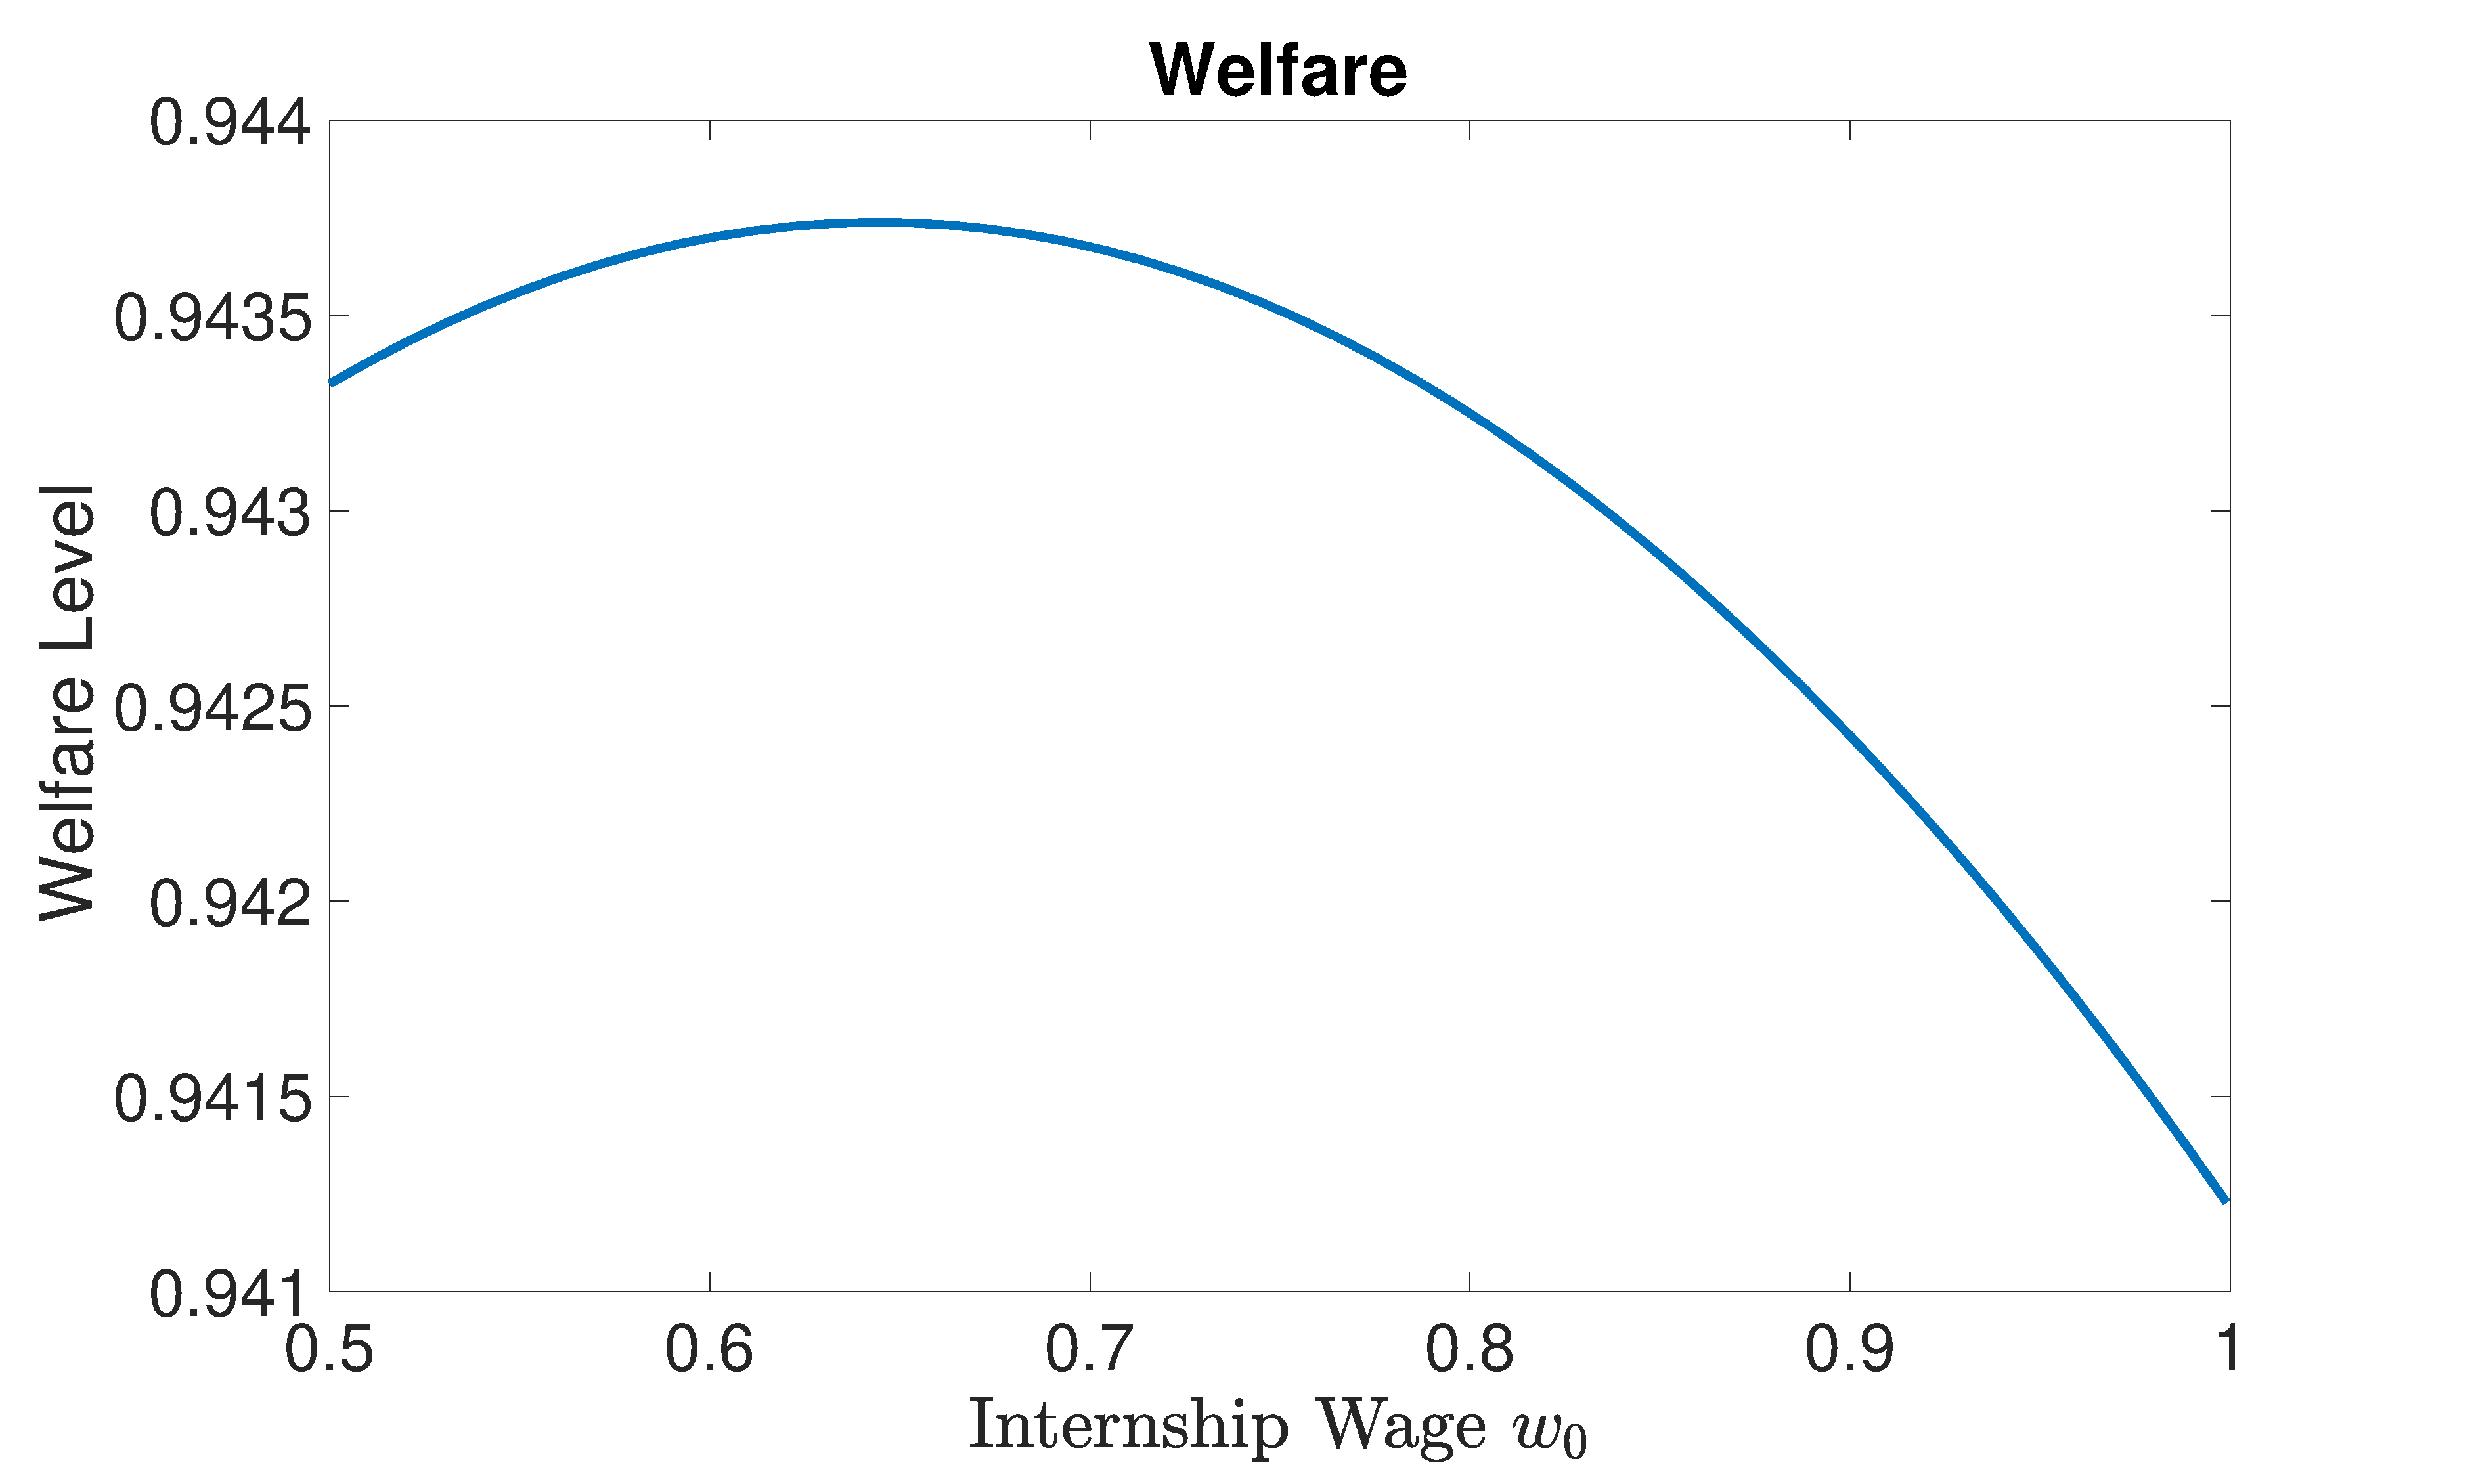
\includegraphics[width=1\linewidth]{welfare_intern.eps}
	\vspace{0em}
	\caption{Aggregate Welfare for Various Levels of Entrant Wages.}
	\label{figure welfare internships}
\end{figure}


Figure \ref{figure welfare internships} graphs the aggregate welfare level for different values of $w_{0}$.
Strikingly, as the entrants' wage increases, aggregate welfare initially increases but after some critical value decreases, yielding an inverse-U shape.
For relatively large values of $w_{0}$, the intervention yields familiar insights: entrants are expensive, firms are discouraged to enter to avoid training costs, and wage increases lead to larger skill loss and lower aggregate welfare.
For relatively low values of $w_{0}$, however, the intervention creates the opposite problem: entrants are too cheap and entry is inefficiently high.
As a result, when $w_{0}$ increases, aggregate welfare also increases because the economy saves in vacancy creation and training costs (this is the well-known reasoning of \citealt{hosios1990efficiency}).
In total, there is a welfare maximizing level of $w_{0}$, which is almost 25\% higher than the corresponding level in the baseline economy.


The most important takeaway is that a carefully designed internship scenario achieves the highest welfare level among all three interventions.
%Intervention 3 brings the economy half way to the constrained efficient welfare level, a non-trivial improvement.
%it comes closest to the planner's treatment by delivering the largest increase in
The reason is that it by delivers the largest increase in the job-finding rate of type-0 workers.
At the same time, every worker type gains from internships other than the experienced type-1 workers.
All in all, these results offer a rationalization of internships in terms of raising aggregate welfare, which may partially explain the popularity of actual internship positions found in modern economies.
%internships cannot make the economy mimic the planner's treatment of the other job-finding rates and that is the reason the economy cannot reach an even higher level of welfare.
%For example, the planner would like a slightly lower $\tilde{f_{1}}$ than the baseline economy, while internships actually help type type-$\tilde{1}$ workers by raising their job-finding rates more than 15\%.
%All in all, it seems that to alleviate the inefficiency found in the baseline economy, more structural changes need to take place in the economy to allow for more flexible interventions with additional degrees of freedom.

\subsection{A fourth intervention} \label{section fourth intervention}

The main message of the discussion in Section \ref{section results} thus far is that government interventions whose goal is to eradicate bias against entrant workers can achieve significant welfare improvements.
The source of these improvements is the reduced unemployment duration of entrant workers which lowers their exposure to skill depreciation shocks and raises aggregate productivity.
In light of this finding, one wonders about the effects of an intervention that ``goes all the way'' and actually induces firms to be biased in favor of entrant workers.
A simple way to achieve this is to consider a government that subsidizes type-0 workers generously enough to tilt the firms' ranking in favor of type-0 over type-1 workers. 
In this environment, matching is still characterized by a \cite{petrongolo2001looking} matching function, but, due to the government's decision to (heavily) subsidize type-0 workers, that worker type is now ranked number one in the firms' preferences. 


More specifically, we consider a government that provides a subsidy $\sigma_0=\kappa(1+\rho)$ to every firm that hires a type-0 worker.\footnote{\,Also, since the subsidy pays for itself, we assume that every firm who is actively producing must pay a flat tax $\tau = \kappa(1+\rho)e_0/e$, which is the direct analogue of equation (\ref{eq tau}).} 
We treat $\rho$ as a parameter that captures the government's generosity and whose value can change. 
But, importantly, any $\rho>0$ implies that firms now rank type-0 workers \textit{first}. 
Under this scenario, the firms' ranking of workers is type $0$ $\succ$ type 1 $\succ$ type $\tilde{1}$ $\succ$ type $\tilde{0}$ and the job-finding rates of the various worker types are very similar to the ones described in Section \ref{section model}. 
The arrival rates, value functions, and the various equilibrium conditions under Intervention 4 are described in detail in Appendix \ref{section appendix intervention 4} for the interested reader. 
We dub this intervention ``type-0 bias'' and present its effects in the last column of Table \ref{table_quantitative_results}.\footnote{\,For this exercise we have set $\rho = 5\%$ because it is small enough to not distort entry incentives too much but still sizeable to incentivize firms to hire type-0 workers.} 

The results of this intervention are striking: it improves aggregate welfare by 1.4\%, more than three times larger than the Internships scenario.
The reason for this sizeable improvement is of course the treatment of type-0 workers, whose job-finding rate quadruples in magnitude.
On the contrary, all other worker types lose from the intervention, since both their job-finding rates and wages substantially decrease, while aggregate unemployment also increases.
The success of Intervention 4 lies on the fact that it directly confronts the problem of type-0 workers spending a lot of time in unemployment upon entry.
As a result, it has the largest impact on the economy's aggregate productivity among all four interventions.
It is important to mention that even though programs of this kind are not popular in the US, they are actually quite common in Europe.
The Youth Employment Initiative, for example, is one of the main financial resources of the European Union to support young people who are not in education or employment.
The total budget of the Youth Employment Initiative was €8.9 billion for the period 2014-2020 to directly finance young workers' apprenticeships, traineeships, job placements, and further education within 4 months of leaving school or becoming unemployed.\footnote{\,The details of the program are available here: \url{https://ec.europa.eu/social/main.jsp?langId=en&catId=89&newsId=9793&furtherNews=yes}.}
Based on our results, interventions of this kind are expected to have large welfare gains, even though they may raise the unemployment rates of other worker groups.



%\begin{equation*}
 %   f_0 = \frac{m(u_0,v)}{u_0} = {b_0}^{\alpha-1}. 
  %  \end{equation*}The three remaining worker types are ``tied for second" in the firms' ranking. To describe their job-finding rate, define $\bar{u_0}\equiv u-u_0$, and $\bar{b_0}=\bar{u_0}/v$.\footnote{\,That is, $\bar{u_0}$ is the measure of all unemployed workers who are not type-0, and $\bar{b_0}$ is the associated queue length. Given the definition of the various queue lengths in equation (\ref{eq queue lengths}), it is obvious that $\bar{b_0}=\tilde{b_0}+b_1+\tilde{b_1}$.} Then, the (common) job-finding rate for all unemployed workers who are not of the preferred type-0 is given by:
%begin{equation*}
%{\bar{f_{0}}}  \left(=f_1=\tilde{f_0}=\tilde{f_1}\right)=\frac{m(u_0+\bar{u_0},v)-m(u_0,v)}{\bar{u_0}} = \frac{(b_0+\bar{b}_0)^\alpha - b_0^\alpha}{\bar{b}_0}. \end{equation*}


\section{Conclusion}\label{section conclusion} 

We develop a DMP model where firms who hire entrant workers have to incur training costs. This allows our model to capture the well-documented bias against entrant workers, as well as the fact that these workers have lower job-finding rates and longer unemployment spells. Entrant workers who stay unemployed for a prolonged period of time are more likely to suffer skill loss, and, motivated by recent findings in the labor economics literature \citep{wachter2020persistent}, we assume that this skill loss has long lasting effects. Our model is characterizes by a prominent market failure. Firms that hire entrant workers provide a \textit{public good} by helping these workers stay unemployed for a shorter period of time, thus mitigating their exposure to the skill loss shock and reducing the measure of ``scarred" workers in the unemployment pool (and the probability that other firms will bump into them). Naturally, however, firms cannot fully internalize this societal contribution, and ultimately choose to discriminate against entrant workers, causing a social welfare loss.  
 
 
Given this market failure, there is obvious scope for government intervention. Since the root of the inefficiency is the inability of firms to fully recoup the training costs, which results in hiring bias against entrants, we consider three government interventions whose common goal is to alleviate the bias and reduce the entrant workers' exposure to the skill loss shock. We use a calibrated version of the model to quantitatively study the effectiveness of three government interventions: ``unbiased matching", ``government subsidies", and ``internships". We find that all three interventions improve aggregate welfare, even though in all of them the aggregate unemployment rate is higher than in the benchmark economy with ranking/bias. The key behind this result is that all government interventions effectively induce firms to incur larger training expenses, thus discouraging entry and increasing unemployment. Despite this unintended consequence on aggregate unemployment, entrant workers have shorter unemployment spells and, as a result, are less likely to suffer skill loss. The productivity gains from the latter channel are so large that aggregate welfare ultimately increases. 

Taking this reasoning to its extreme, we consider a fourth intervention in which the government subsidizes the hiring of entrant workers so heavily that firms actually rank these workers higher than the experienced ones. 
This intervention delivers a substantial improvement in aggregate welfare, at least three times larger than the other three interventions, because it directly confronts the problem of inexperienced workers spending a lot of time in unemployment upon entry.
Hence, our analysis predicts that programs that promote the training and job-placement of young workers, such as the Youth Employment Initiative in the EU, generate sizeable welfare gains.


%In terms of quantitative results, we find that Intervention 1, which imposes unbiased matching by law, increases welfare by 0.38\%, compared to the baseline model. Intervention 2 achieves unbiased matching by taxing all active matches and using the revenues to subsidize firms who hire entrant workers. Under this intervention the welfare increase is smaller, around 0.31\%, because the tax needed to finance training subsidies reduces the match surplus and further distorts entry. Under Intervention 3, entrant workers' wages are exogenous and we treat them as parameters whose level varies. For high wages, entrant workers are compensated almost as much as they would under Nash bargaining, so Intervention 3 becomes virtually equivalent to Intervention 1. On the other extreme, if entrant wages are low, firms realize they can hire these workers almost for free, which leads to excessive entry and large levels of training and vacancy creation costs. We show that aggregate welfare is maximized for intermediate levels of entrant wage, and it can go up to 0.42\% above the baseline model. In conclusion, a carefully designed internship scenario achieves the highest welfare among all interventions.

%We need a few words about the comparison of the various interventions with the SPP. 

\newpage


\setlength{\bibsep}{0pt}
%\bibliography{GHS}

\bibliography{AGKbib} 

\newpage

\begin{appendix}

% format the equation environment
\renewcommand{\theequation}{A.\arabic{equation}}

% reset the counter
\setcounter{equation}{0}

\section{Appendix: Proofs of Results}\label{section appendix proofs}
\begin{proof}{Derivation of the job-finding rates for each type of workers.}

\noindent Using the formula for a CRS Cobb-Douglas matching function and the usual notations for the variables, the job-finding rate for a worker of type 1 is given by: 
\begin{eqnarray*}
     f_1 = \frac{m(u_1,v)}{u_1} =  \frac{u_1^\alpha v^{1-\alpha}}{u_1^\alpha u_1^{1-\alpha}}  = {b_1}^{\alpha-1}.  
\end{eqnarray*}
Now, for the type-$\tilde{1}$ workers, one can use the \cite{petrongolo2001looking} logic that type-1 workers “move first”, and, only then, type-$\tilde{1}$ workers get a chance to match. The authors of that paper capture this idea by subtracting the matches of only type-${1}$ workers (the ``first movers") from the total matches of type-1 and type-$\tilde{1}$ workers, i.e.,  
\begin{eqnarray*}
     \tilde{f_1} &=& \frac{m(u_1+\tilde{u_1},v)-m(u_1,v)}{\tilde{u_1}} \\
      &=& \frac{(u_1+\tilde{u_1})^\alpha v^{1-\alpha}}{\tilde{u_1}} -\frac{u_1^\alpha v^{1-\alpha}}{\tilde{u_1}} \\
        &=& \left(\frac{u_1+\tilde{u_1}}{v}\right)^{\alpha} \cdot \frac{v}{\tilde{u_1}} - \left(\frac{u_1}{v}\right)^{\alpha}\cdot  \frac{v}{\tilde{u_1}}  \\
        &=& \frac{(b_1+\tilde{b}_1)^\alpha - b_1^\alpha}{\tilde{b}_1}.
\end{eqnarray*}The derivations for the job-finding rates of type-0 and type-$\tilde{0}$ workers follow similar steps, hence, they are omitted. But the logic of matching with ranking based on \cite{petrongolo2001looking} is exactly the same, adjusted for a richer set of types. 

Based on the \cite{petrongolo2001looking} method, and following similar steps, we can also derive the various worker-finding rates for firms. (These are the $q$ expressions that appear in the job creation curves.) Specifically, we have:  
\begin{eqnarray*}
q_1 &=& b_1^\alpha, \\
\tilde{q_1} &=&  (b_1+\tilde{b_1})^\alpha - b_1^\alpha, \\
q_0 &=& (b_1+\tilde{b_1}+b_0)^\alpha - (b_1+\tilde{b_1})^\alpha, \\
\tilde{q_0} &=&  (b_1+b_0+\tilde{b_1}+\tilde{b_0})^\alpha - (b_1+b_0+\tilde{b_1})^\alpha.
\end{eqnarray*}
\end{proof}

\begin{proof}{Proof of Lemma \ref{lemma all ws the same}.}
Since the various $J_i$ terms are all equal to each other, and since the bargaining problem in each type of meeting will imply $(1-\eta)(W_i-U_i)=\eta J_i$, we must have that the various $W_i-U_i$ terms are also equal to each other. Let us subtract $U_1$, given by equation (\ref{eq U1 inter 1}), from $W_1$, given by equation (\ref{eq W1}); this will give us 
\begin{equation}
W_1-U_1=\frac{w_1-z}{r+\lambda+\delta+f}. \label{eq W1 - U1}
\end{equation}Similarly, let us subtract $\tilde{U_1}$, given by equation (\ref{eq U1 tilde inter 1}), from $\tilde{W_1}$, given by equation (\ref{eq W1 tilde}); this will give us 
\begin{equation}
\tilde{W_1}-\tilde{U_1}=\frac{\tilde{w_1}-z}{r+\lambda+\delta+f}. \label{eq W1 - U1 tilde} 
\end{equation}Direct comparison of equations (\ref{eq W1 - U1}) and (\ref{eq W1 - U1 tilde}), implies that $w_1=\tilde{w_1}$. 

Next, subtract $\tilde{U_0}$, given by equation (\ref{eq U0 tilde inter 1}), from $\tilde{W_0}$, given by equation (\ref{eq W0 tilde}), to obtain 
\begin{equation}
 (r+\delta+f)(\Tilde{W_0}-\Tilde{U_0})=\Tilde{w_0}-z+\lambda(\Tilde{U_1}-\Tilde{W_0}). \label{eq W0 - U0 tilde aux}
\end{equation}To obtain a useful expression for the term $\Tilde{U_1}-\Tilde{W_0}$ in the last equation, subtract $\Tilde{W_0}$, given by equation (\ref{eq W0 tilde}), from $\Tilde{U_1}$, given by equation (\ref{eq U1 tilde inter 1}). This will give us   
\begin{equation}
(r+\delta+\lambda)(\Tilde{U_1}-\Tilde{W_0})=z-\Tilde{w_0}+f(\Tilde{W_1}-\Tilde{U_1}), \nonumber 
\end{equation}which we can now use to replace the term $\Tilde{U_1}-\Tilde{W_0}$ in equation (\ref{eq W0 - U0 tilde aux}). After this substitution, one should find that 
\begin{equation*}
(r+\delta+f)(\Tilde{W_0}-\Tilde{U_0})=(\Tilde{w_0}-z)\left(1-\frac{\lambda}{r+\delta+\lambda}\right) + \frac{\lambda f}{r+\delta+\lambda}(\Tilde{W_1}-\Tilde{U_1}).
\end{equation*}But since we have already established that $(\Tilde{W_0}-\Tilde{U_0})=(\Tilde{W_1}-\Tilde{U_1})$, the last equation can be re-written as 
\begin{equation*}
   \left(r+\delta+f-\frac{\lambda f}{r+\delta+\lambda}\right)(\Tilde{W_0}-\Tilde{U_0})=\Tilde{w_0}-z+\frac{r+\delta}{r+\delta+\lambda},  
\end{equation*}which, after some algebra, simplifies to  
\begin{equation}
      \Tilde{W_0}-\Tilde{U_0} = \frac{\Tilde{w_0}-z}{r+\delta+\lambda+f}.\label{eq W0 - U0 tilde}  
\end{equation}Direct comparison of equations (\ref{eq W1 - U1}), (\ref{eq W1 - U1 tilde}), and (\ref{eq W0 - U0 tilde}), implies that $w_1=\tilde{w_1}=\Tilde{w_0}$.

The last thing is to show that the remaining wage $w_0$ is also equal to the wages of the other three types. To that end, start by subtracting subtract ${U_0}$, given by equation (\ref{eq U0 inter 1}), from ${W_0}$, given by equation (\ref{eq W0}), to obtain 
\begin{equation}
(r+\delta+f)(W_0-U_0)=w_0-z+\lambda(U_1-W_0)+\gamma(U_0-\Tilde{U_0}).\label{eq W0 - U0 aux} 
\end{equation}Again, we can find more useful expressions for the terms $U_1-W_0$ and $U_0-\Tilde{U_0}$ in the last equation. Subtracting $W_0$, given by equation (\ref{eq W0}), from $U_1$, given by equation (\ref{eq U1 inter 1}), we get 
\begin{equation*}
   (r+\delta+\lambda)(U_1-W_0)=z-w_0+f(W_1-U_1).
  \end{equation*}
As for the term $U_0-\Tilde{U_0}$, it is easy to show that 
\begin{equation*} 
(r+\delta+\gamma)(U_0-\Tilde{U_0})=0 \implies U_0=\Tilde{U_0}. 
\end{equation*}Using these two facts back into equation (\ref{eq W0 - U0 aux}) allows to write  
\begin{equation}
(r+\delta+f)(W_0-U_0)=w_0-z+\frac{\lambda}{r+\delta+\lambda}[z-w_0+f(W_1-U_1)].\nonumber 
\end{equation}But since we have established that $(W_0-U_0)=(W_1-U_1)$, the last equation can be re-written as \begin{equation*}
   \left(r+\delta+f-\frac{\lambda f}{r+\delta+\lambda}\right)(W_0-U_0)=(w_0-z)\cdot \frac{r+\delta}{r+\delta+\lambda},  
   \end{equation*}which, after some algebra, simplifies to  
\begin{equation}
      W_0-U_0 = \frac{w_0-z}{r+\delta+\lambda+f}.\label{eq W0 - U0}  
\end{equation}Comparison of equations (\ref{eq W1 - U1}), (\ref{eq W1 - U1 tilde}), (\ref{eq W0 - U0 tilde}), and (\ref{eq W0 - U0}) implies that $w_1=\tilde{w_1}=\Tilde{w_0}=w_0$, which concludes the proof.\end{proof} 


%%%%%%%%%%%%%%%%%%%%%%%%%%%%%%%%%%%%%%%%%%%%%%%%%%%%%%%%%%%%%%%%%%%%%%%%%%%%%%%%%%%%%%%%%%%%%%%%%%%%%%%%%%%%%%%%%%%%%%%%%%%%%%%%%%%%%%%%%%%%%%%%%%%%%%%%%%%%%%%%%%%%%%%%%%%%%%%%%%%%%%%%%%%%%%%%%%%%%%%%%%%%%%%%%%%%%%%%%%%%%%%%%%%%%%%%%%%%%%%%

\iffalse


\begin{proof}{Proof of Lemma \ref{lemma SPP}.}
Similar to the Chapter 8 of \cite{pissarides2000equilibrium}, we can set up the Hamiltonian based on the SPP with various $\dot{\mu}_0$'s as co-state variables. Then, we derive the first order conditions by setting the derivatives of the Hamiltonian with respect to the market tightness equal to zero and the derivatives with respect to the various employment states equal to the negative of the evolution of the respective co-state variables. Following the steps, we get the following 12 equations for the first order conditions:

\begin{eqnarray}
    \frac{\partial \mathcal{H}}{\partial \theta_0} &=& 0 \iff ce^{-rt}=(1-\alpha){\theta_0}^{-\alpha} (\mu_{e_0}-\mu_{u_0}), \label{foc1} \\
    \frac{\partial \mathcal{H}}{\partial \theta_1} &=& 0 \iff ce^{-rt}=(1-\alpha){\theta_1}^{-\alpha} (\mu_{e_1}-\mu_{u_1}), \label{foc2}\\
     \frac{\partial \mathcal{H}}{\partial \tilde{\theta_0}} &=& 0 \iff ce^{-rt}=(1-\alpha){\tilde{\theta_0}}^{-\alpha} (\mu_{\tilde{e_0}}-\mu_{\tilde{u_0}}), \label{foc3}\\
      \frac{\partial \mathcal{H}}{\partial \tilde{\theta_1}} &=& 0 \iff ce^{-rt}=(1-\alpha){\tilde{\theta_1}}^{-\alpha} (\mu_{\tilde{e_1}}-\mu_{\tilde{u_1}}), \label{foc4}\\
      \frac{\partial \mathcal{H}}{\partial u_0} &=& -\dot{\mu}_{u_0} \iff e^{-rt}(z-c\theta_0)-\mu_{u_0}(\delta+\gamma+f_0)+\mu_{\tilde{u_0}}\gamma + \mu_{e_0}f_0= -\dot{\mu_{u_0}}, \label{foc5}\\
       \frac{\partial \mathcal{H}}{\partial u_1} &=& -\dot{\mu}_{u_1} \iff e^{-rt}(z-c\theta_1)-\mu_{u_1}(\delta+f_1) + \mu_{e_1}f_1 = -\dot{\mu_{u_1}}, \label{foc6}\\
       \frac{\partial \mathcal{H}}{\partial \tilde{u_0}} &=& -\dot{\mu}_{\tilde{u_0}} \iff e^{-rt}(z-c\tilde{\theta_0})-\mu_{\tilde{u_0}}(\delta+\tilde{f_0}) + \mu_{\tilde{e_0}}\tilde{f_0} = -\dot{\mu}_{\tilde{u_0}}, \label{foc7}\\
      \frac{\partial \mathcal{H}}{\partial \tilde{u_1}} &=& -\dot{\mu}_{\tilde{u_1}} \iff e^{-rt}(z-c\tilde{\theta_1})-\mu_{\tilde{u_1}}(\delta+\tilde{f_1}) + \mu_{\tilde{e_1}}\tilde{f_1} = -\dot{\mu}_{\tilde{u_1}}, \label{foc8}\\ 
      \frac{\partial \mathcal{H}}{\partial e_0}  &=& -\dot{\mu}_{e_0} \iff e^{-rt}(p-\kappa)+\mu_{u_1} \lambda -\mu_{e_0}(\delta + \lambda) = -\dot{\mu}_{e_0}, \label{foc9}\\
       \frac{\partial \mathcal{H}}{\partial e_1}  &=& -\dot{\mu}_{e_1} \iff e^{-rt}p+\mu_{u_1} \lambda -\mu_{e_1}(\delta + \lambda) = -\dot{\mu}_{e_1}, \label{foc10}\\
        \frac{\partial \mathcal{H}}{\partial \tilde{e_0}}  &=& -\dot{\mu}_{\tilde{e_0}} \iff e^{-rt}(p-\kappa-\tilde{\kappa})+\mu_{\tilde{u_1}} \lambda -\mu_{\tilde{e_0}}(\delta + \lambda) = -\dot{\mu}_{\tilde{e_0}}, \label{foc11}\\
         \frac{\partial \mathcal{H}}{\partial \tilde{e_1}}  &=& -\dot{\mu}_{\tilde{e_1}} \iff e^{-rt}(p-\kappa)+\mu_{\tilde{u_1}} \lambda -\mu_{\tilde{e_1}}(\delta + \lambda) = -\dot{\mu}_{\tilde{e_1}}. \label{foc12}
\end{eqnarray}
We use the above first order conditions to get the final four SPP equations in Lemma \ref{lemma SPP}. For the first equation (\ref{eq theta 1}), subtracting equation (\ref{foc10}) from (\ref{foc6}) gives:
\begin{equation}
   \dot{\mu}_{e_1}-\dot{\mu}_{u_1}=(\delta + \lambda+f_1)(\mu_{e_1}-\mu_{u_1})-e^{-rt}(p-z+c\theta_1). \label{intermed1}
\end{equation}
From equation (\ref{foc2}), we have
\begin{eqnarray*}
 \mu_{e_1}-\mu_{u_1} = \frac{ce^{-rt}}{(1-\alpha){\theta_1}^{-\alpha}} \implies  \dot{\mu}_{e_1}-\dot{\mu}_{u_1} = \frac{-cre^{-rt}}{(1-\alpha){\theta_1}^{-\alpha}}.
\end{eqnarray*}
Plugging this to equation (\ref{intermed1}) along with some algebra yields equation (\ref{eq theta 1}). 

Then, the second equation (\ref{eq theta 1 tilde}) can be obtained by subtracting equation (\ref{foc12}) from (\ref{foc8}) and using similar steps. In this case, we use equation (\ref{foc4}) to obtain useful expressions for $\mu_{\tilde{e_1}}-\mu_{\tilde{u_1}}$ and $\dot{\mu}_{\tilde{e_1}}-\dot{\mu}_{\tilde{u_1}}$ to get the final equation. 

For the third equation (\ref{eq theta 1 tilde}), the steps are slightly more involved because when we subtract (\ref{foc11}) from (\ref{foc7}), we obtain:
\begin{equation}
   \dot{\mu}_{\tilde{e_0}}-\dot{\mu}_{\tilde{u_0}}=(\delta + \tilde{f_0})(\mu_{\tilde{e_0}}-\mu_{\tilde{u_0}}) + \lambda(\mu_{\tilde{e_0}}-\mu_{\tilde{u_1}})-e^{-rt}(\tilde{p}-z+c\tilde{\theta_0}). \label{intermed2}
\end{equation}
Here, $\dot{\mu}_{\tilde{e_0}}-\dot{\mu}_{\tilde{u_0}}$ and $\mu_{\tilde{e_0}}-\mu_{\tilde{u_0}}$ can be obtained from equation (\ref{foc3}) using similar steps as before. For $\mu_{\tilde{e_0}}-\mu_{\tilde{u_1}}$, use equation (\ref{foc8}) to get:
\begin{equation}
    e^{-rt}(z-c\tilde{\theta_1}) + \tilde{f_1}(\mu_{\tilde{e_1}}-\mu_{\tilde{u_1}}) = (r+\delta){\mu}_{\tilde{u_1}}. \label{intermed3}
\end{equation}
Similarly from equation (\ref{foc11}), we get:  
\begin{equation}
    e^{-rt}(p-\kappa-\tilde{\kappa})+\mu_{\tilde{u_1}} \lambda = \mu_{\tilde{e_0}}(r + \delta + \lambda). \label{intermed4}
\end{equation}
Subtracting equation (\ref{intermed3}) from (\ref{intermed4}) and substituting in equation (\ref{intermed2}) followed by some algebraic manipulations yield the final equation (\ref{eq theta 1 tilde}) involving $\tilde{\theta_0}$ and $\tilde{\theta_1}$. 

The steps to derive the final equation (\ref{eq theta 0}) are similar to the steps above for the third equation. We first subtracted equation (\ref{foc9}) from (\ref{foc5}). Similar to before, we subtract the expressions obtained from equations (\ref{foc6}) and (\ref{foc9}) to get $\mu_{e_0}-\mu_{u_1}$, and we subtract the expressions obtained from equations (\ref{foc5}) and (\ref{foc7}) to get $\mu_{\tilde{u_0}}-\mu_{u_0}$. Substituting all the expressions followed by some algebra yields equation (\ref{eq theta 0}).
\end{proof}

\fi

%%%%%%%%%%%%%%%%%%%%%%%%%%%%%%%%%%%%%%%%%%%%%%%%%%%%%%%%%%%%%%%%%%%%%%%%%%%%%%%%%%%%%%%%%%%%%%%%%%%%%%%%%%%%%%%%%%%%%%%%%%%%%%%%%%%%%%%%%%%%%%%%%%%%%%%%%%%%%%%%%%%%%%%%%%%%%%%%%%%%%%%%%%%%%%%%%%%%%%%%%%%%%%%%%%%%%%%%%%%%%%%%%%%%%%%%%%%%%%%%





\section{Appendix: The details of Intervention 4 \label{section appendix intervention 4}}

This appendix contains the details of the analysis under ``Intervention 4", i.e., a government subsidy \textit{only} to type-0 workers, which is generous enough to make them the preferred types for firms. 

\medskip 

\noindent \textbf{Arrival rates and Beveridge curves}

\medskip 

\noindent As we discussed in the main body of the paper, we will still have a \cite{petrongolo2001looking} matching process, but the ranking will now favor type-0 workers. (The relative ranking of the remaining types will stay unchanged.) Recalling the definition of the various {queue lengths}, from equation (\ref{eq queue lengths}), one can easily show that the new job-finding rates for the four worker types are as follows: 
\begin{eqnarray*}
	f_0 &=& \frac{m(u_0,v)}{u_0} = {b_0}^{\alpha-1}, \\
	{f_1} &=& \frac{m(u_0+{u_1},v)-m(u_0,v)}{{u_1}} = \frac{(b_0+{b}_1)^\alpha - b_0^\alpha}{{b}_1}, \\
	\tilde{f_1} &=& \frac{m(u_0+u_1+\tilde{u_1},v)-m(u_0+{u_1},v)}{\tilde{u_1}} = \frac{(b_0+{b}_1+\tilde{b_1})^\alpha - (b_0+{b}_1)^\alpha}{\tilde{b_1}}, \\
	\tilde{f}_0 &=& \frac{m(u_0+u_1+\tilde{u_1}+\tilde{u_0},v)-m(u_0+u_1+\tilde{u_1},v)}{\tilde{u_0}} = \frac{(b_0+b_1+\tilde{b}_1+\tilde{b}_0)^\alpha - ({b_0+b_1+\tilde{b}_1})^\alpha}{\tilde{b}_0}. 
\end{eqnarray*}The formulas admit an interpretation similar to the one provided in Section \ref{section model}. Although the job-finding rates have changed to reflect the new ranking of workers, the formulas describing the Beveridge curves in Section \ref{section beveridge} are still valid.  

Next, following similar steps, we can derive the various worker-finding rates for firms. These are given by:  
\begin{eqnarray*}
	q_0 &=& b_0^\alpha, \\
	{q_1} &=&  (b_0+{b_1})^\alpha - b_0^\alpha, \\
	\tilde{q_1} &=& (b_0+b_1+\tilde{b_1})^\alpha - (b_0+{b_1})^\alpha, \\
	\tilde{q_0} &=&  (b_0+b_1+\tilde{b_1}+\tilde{b_0})^\alpha - (b_0+b_1+\tilde{b_1})^\alpha.
\end{eqnarray*}

\medskip 

\noindent \textbf{Value functions and free entry}

\medskip 

\noindent Since in equilibrium we must have $V=0$, we can state the free entry condition as 
\begin{equation}
c= q_0 J_0 + \Tilde{q_0}\Tilde{J_0} + q_1 J_1 + \Tilde{q_1}\Tilde{J_1}, \label{eq free entry intervention 4} 
\end{equation}where the value functions for productive firms in the various states are as follows: \begin{eqnarray*}rJ_0 &=&p+\kappa \rho- \tau  -w_0-\lambda J_0 - \delta J_0,\label{eq J0} \\
	r\Tilde{J_0} &=&p-\kappa-\Tilde{\kappa}- \tau -\Tilde{w_0}-\lambda \Tilde{J_0} - \delta \Tilde{J_0},\label{eq J0 tilde}\\
	rJ_1 &=&p- \tau -w_1-\lambda J_1 - \delta J_1, \label{eq J1} \\
	r\Tilde{J_1} &=&p-\Tilde{\kappa}-\tau-\Tilde{w_1}-\lambda \Tilde{J_1} - \delta \Tilde{J_1} . \label{eq J1 tilde}
\end{eqnarray*}Clearly, the difference of these value functions with the ones provided in Section \ref{section analysis} is that firms who hire type-0 workers are better off, due to the government subsidy (equal to $\sigma_0=\kappa (1+\rho)$), and that all active firms pay the flat tax $\tau$.\footnote{\,Which, in equilibrium, will be equal to $\tau = \kappa(1+\rho)e_0/e$, in order to keep the government budget constraint balanced.} 

The value functions of unemployed workers in the various states are still given by equations (\ref{eq U0})-(\ref{eq U1 tilde}), even though the respective job-finding rates have now changed. Similarly, the value functions of employed workers in the various states are still described by equations (\ref{eq W0})-(\ref{eq W1 tilde}).

\medskip 

\noindent \textbf{Bargaining and wage curves}

\medskip 

\noindent Deriving the various wage curves follows identical steps to the analysis in Section \ref{section bargaining}. We will therefore skip the details and proceed to the final formulas. The careful reader will observe that the following wage curves look identical to the ones provided in Section \ref{section bargaining}, after adjusting the formulas to reflect the new productivities.\footnote{\,Namely, the fact that all firms must now pay a tax, and that firms that match with type-0 workers receive a subsidy which makes the pre-tax effective productivity of these workers equal to $p+\kappa \rho$.} More precisely, we have:    
\begin{equation*}
w_1 = \frac{\eta (p-\tau) (r+\delta+\lambda+f_1)+(1-\eta)z(r+\delta+\lambda)}{r+\delta+\lambda + \eta f_1},  
\end{equation*}
\begin{equation*}
\Tilde{w_1} = \frac{\eta (p-\Tilde{\kappa}-\tau) (r+\delta+\lambda+\tilde{f_1})+(1-\eta)z(r+\delta+\lambda)}{r+\delta+\lambda + \eta \tilde{f_1}},  
\end{equation*}
\begin{equation*} 
\Tilde{w_0} = \frac{1}{r+\delta+\eta \Tilde{f_0}}\left[\eta(p-\kappa-\Tilde{\kappa}-\tau)(r+\delta+ \Tilde{f_0})+\frac{(r+\delta+\lambda)(r+\delta+\Tilde{f_1})}{r+\delta+\lambda+\Tilde{f_1}}(1-\eta)z - \frac{\lambda(1-\eta)\Tilde{f_1}}{r+\delta+\lambda+\Tilde{f_1}}\Tilde{w_1} \right].
\end{equation*}
%\begin{equation*} \label{eq WC0 tilde inter 1}
%%\hspace{-1cm}\Tilde{w_0}  = \frac{r+\delta+ \tilde{f_0}}{r+\delta+\eta {f}} 
%%\left[\eta(p-\kappa-\Tilde{\kappa}) +\frac{r+\delta+\lambda}{r+\delta+\lambda+f}(1-\eta)z - \frac{\lambda(1-\eta){f}}{(r+\delta+\lambda+f)(r+\delta+ f)}\Tilde{w_1} \right],
%%\end{equation*}
\begin{equation*}
\begin{split}
w_0 & = \frac{r+\delta+\gamma +f_0}{r+\delta+\gamma+\eta f_0}\eta (p+\kappa \rho -\tau) + \frac{(r+\delta +\lambda)(r+\delta+f_1)(r+\delta+\gamma)}{(r+\delta)(r+\delta+\gamma + \eta f_0)(r+\delta+\lambda+f_1)} (1-\eta) z  \\  
& + \frac{\gamma \Tilde{f_0}\eta(p-\kappa-\Tilde{\kappa}-\tau -\Tilde{w_0})}{(r+\delta)(r+\delta+\gamma + \eta f_0)} - \frac{(1-\eta)\lambda f_1 (r+\delta+\gamma)w_1}{(r+\delta)(r+\delta+\gamma + \eta f_0)(r+\delta+\lambda+f_1)}. 
\end{split}
\end{equation*}

\medskip

\begin{definition}\label{definition equilibrium}
	A steady state equilibrium under Intervention 4 is a list of wages for the four types of workers $(w_0, \Tilde{w_0}, w_1, \Tilde{w_1})$, a measure of vacant firms $v$, and measures of unemployed and employed workers in the various states $(u_0, \Tilde{u_0}, u_1, \Tilde{u_1}, e_0, \Tilde{e_0}, e_1, \Tilde{e_1})$, satisfying the free entry condition (\ref{eq free entry intervention 4}), the four wage curves described in this section, and the eight Beveridge curves reported at the end of Section \ref{section beveridge}. Implicit in this definition is the flat tax paid by all active firms, given by $\tau = \kappa(1+\rho)e_0/e$. 
\end{definition} 





%\section{Appendix: A version of the model without scar}\label{section appendix no scar}
%
%\subsection{Analysis of the model without scar}\label{section analysis no scar}
%In the main part of this paper, we worked with the ``model with skill loss \textbf{and} scar" in which entrant workers who stay unemployed for a prolonged period of time if hit by a skill loss shock get permanently scarred affecting their productivity for their lifetime. Here, we present the version of the ``model with skill loss \textbf{but without any} scar". All the variables and parameters are similar to the main model except the key difference that the skill loss does not scar the workers permanently; once they have been employed at least once and then lose their job, all types of workers end up in the same pool of unemployed workers ($u_1$ in the below figure) and have no permanent difference in productivity.
%\begin{figure}[h]
%	\centering
%	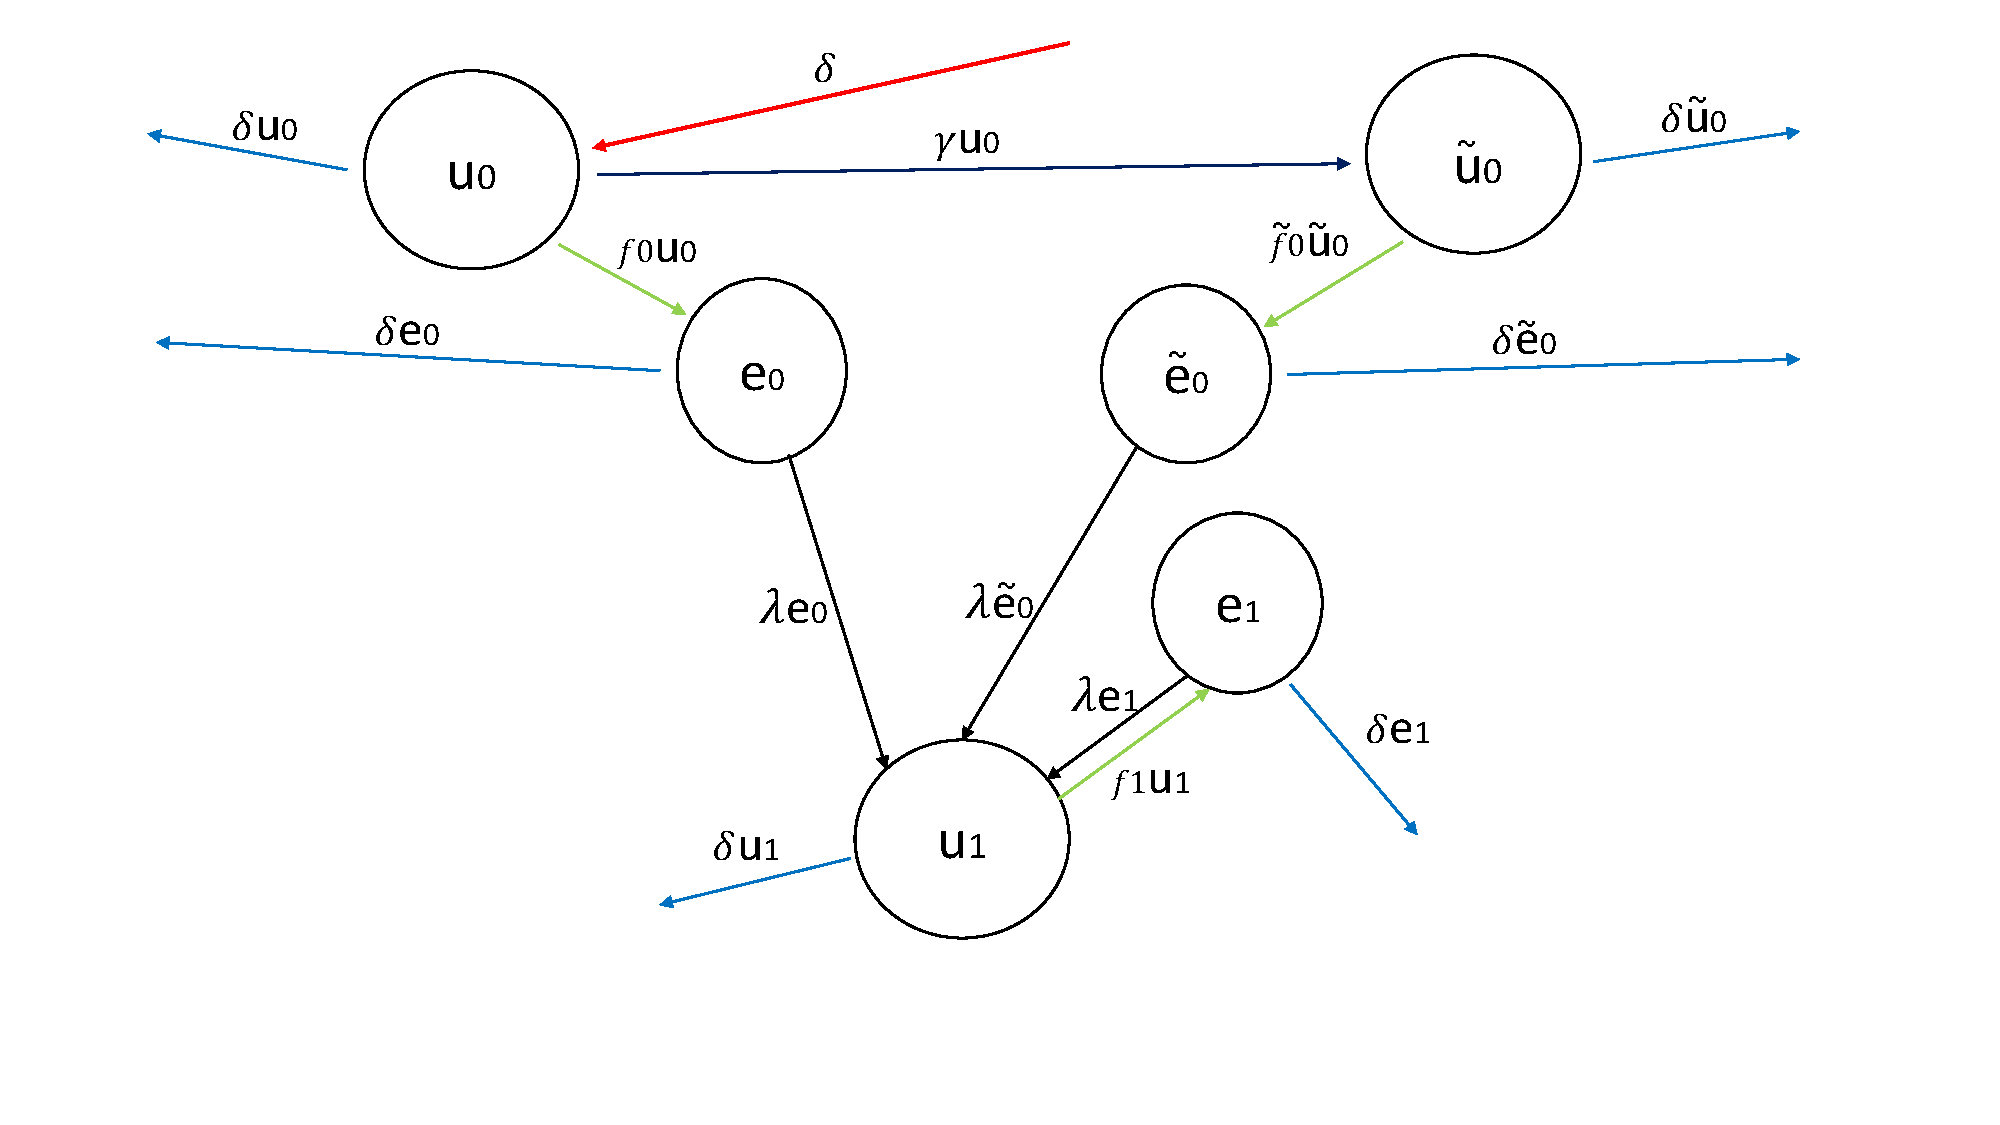
\includegraphics[width=1.05\linewidth]{empl_states_no_scar.pdf}
%	\vspace{0em}
%	\caption{Worker flows in and out of the various states (model with no scar).}
%	\label{figure model no scar}
%\end{figure}
%
%\subsubsection{Beveridge curves}\label{section beveridge no scar}
%To derive the Beveridge curves, we can look at above figure, which illustrates the worker flows in and out of every state in the environment without any scar. The graph is a simplified version of figure 1, so the interpretation is similar. Equating the flows in and out of the various states and after some algebra, we find the following steady state measure of workers in the various states:   
%\begin{eqnarray*}
%u_0 &=& \frac{\delta}{\delta+\gamma+f_0},  \\
%\tilde{u_0} &=& \frac{\gamma}{\delta+\Tilde{f_0}} \cdot  \frac{\delta}{\delta+\gamma+f_0},   \\
%u_1 &=& \frac{\lambda(\gamma\Tilde{f_0}+\delta f_0 + f_0\Tilde{f_0})}{(\delta+\Tilde{f_0})(\delta+\gamma+f_0)(\delta + \lambda + f_1)} , \\
%e_0 &=& \frac{f_0}{\delta+\lambda} \cdot \frac{\delta}{\delta+\gamma+f_0}, \\
%\Tilde{e_0} &=& \frac{\Tilde{f_0}}{\delta+\lambda} \cdot \frac{\gamma}{\delta + \Tilde{f_0}} \cdot \frac{\delta}{\delta+\gamma+f_0}, \\
%e_1 &=& \frac{f_1}{\delta+\lambda} \cdot \frac{\lambda(\gamma\Tilde{f_0}+\delta f_0 + f_0\Tilde{f_0})}{(\delta+\Tilde{f_0})(\delta+\gamma+f_0)(\delta + \lambda + f_1)}.
%\end{eqnarray*}
%
%\subsubsection{Value Functions}\label{section value functions no scar}
%Next, we find the steady state value functions similar to before. We start with a vacant firm with $q$ as its arrival rate of workers to firms:
%\begin{equation*}
%   rV = -c + q_0 (J_0-V) + \Tilde{q_0}(\Tilde{J_0}-V) + q_1 (J_1-V).
%\end{equation*}The free entry implies that $V=0$ in equilibrium, so, the above free entry condition becomes 
%\begin{equation}
%   c = q_0J_0 + \Tilde{q_0}\Tilde{J_0} + q_1J_1.\label{eq free entry no scar} 
%\end{equation}
%
%We have three value functions for productive firms in the various states, i.e., for firms who matched with the three different types of workers (type 0, $\tilde{0}$, and 1). 
%\begin{eqnarray}
%     rJ_0 &=& p-\kappa-w_0-\lambda J_0 - \delta J_0, \label{eq J0 no scar} \\
%     r\Tilde{J_0} &=& p-\kappa-\Tilde{\kappa}-\Tilde{w_0}-\lambda \Tilde{J_0} - \delta \Tilde{J_0}, \label{eq J0 tilde no scar} \\
%    rJ_1 &=& p-w_1-\lambda J_1 - \delta J_1. \label{eq J1 no scar} 
%    \end{eqnarray}
%
%Now, we move on to the value functions of workers in the various states. All the notations are standard. The value functions for unemployed workers in the various states are given by: 
%\begin{eqnarray}
%    rU_0 &=& z+f_0(W_0-U_0)+\gamma(\Tilde{U_0}-U_0) - \delta U_0, \label{eq U0 no scar} \\
%     r\Tilde{U_0} &=& z+\Tilde{f_0}(\Tilde{W_0}-\Tilde{U_0})- \delta \Tilde{U_0},
%     \label{eq U0 tilde no scar} \\
%    rU_1 &=& z+f_1(W_1-U_1)- \delta U_1. \label{eq U1 no scar} 
%\end{eqnarray}
%The value functions for employed workers in the various states are given by: 
%\begin{eqnarray}
%    rW_0 &=&w_0+\lambda(U_1-W_0)- \delta W_0, \label{eq W0 no scar} \\
%     r\Tilde{W_0} &=& \Tilde{w_0}+\lambda(U_1-\Tilde{W_0})- \delta \Tilde{W_0},  \label{eq W0 tilde no scar} \\
%     rW_1 &=& w_1+\lambda(U_1-W_1)- \delta W_1. \label{eq W1 no scar} 
%     \end{eqnarray}
%Similar to before any inexperienced workers who lose their first job move to the pool of experienced unemployed workers, so the term $U_1$ appears on the right-hand side of equations for $W_0$ and $\Tilde{W_0}$.
%
%Now, we have all the value functions for the firms and workers, we can move to the bargaining problems in the various types of meetings in this environment without any scar. 
%
%\subsubsection{Bargaining problems}\label{section bargaining no scar} 
%\textbf{Bargaining in type-1 meeting}
%
%\medskip 
%
%\noindent Like in the case for the model with scar, solving the standard Nash bargaining problem between a firm and an unemployed worker of type-1 implies that the following condition must be satisfied:
%\begin{equation}
%(1-\eta)(W_1-U_1) = \eta J_1. \label{eq bargain 1 no scar}
%\end{equation}
%Following similar steps as before, we use the value functions for $W_1$, $J_1$, and $U_1$ from (\ref{eq W1 no scar}, \ref{eq J1 no scar}, and \ref{eq U1 no scar} respectively) to get the following equation for the ``wage curve" for type-1 workers in this environment with no scar. 
%\begin{equation}
% w_1 = \frac{\eta p (r+\lambda+\delta+f_1)+(1-\eta)z(r+\lambda+\delta)}{r+\lambda+\delta + \eta f_1}. \label{eq WC1 no scar}
%\end{equation} Note that the equation is identical to wage curve in the model with scar. 
%
%\bigskip 
%
%\noindent \textbf{Bargaining in type-$\Tilde{0}$ meeting}
%
%\medskip 
%
%\noindent The surplus sharing rule between an inexperienced worker who suffered skill loss and a firm is given by the following equation:
%\begin{equation}
%       (1-\eta)(\Tilde{W_0}-\Tilde{U_0}) = \eta \Tilde{J_0}.  \label{eq bargain 0 tilde no scar}
%\end{equation}Same as before, we replace the value functions $\tilde{W_0}$ and $\tilde{J_0}$ from (\ref{eq W0 tilde no scar}) and (\ref{eq J0 tilde no scar}), respectively, to write the wage of a type-$\tilde{0}$ worker as
%\begin{equation}
%   \Tilde{w_0} = \eta (p-\kappa-\Tilde{\kappa})  - \lambda (1-\eta)(U_1 - \Tilde{U_0}) + (1-\eta)(r+\delta) \Tilde{U_0} . \label{eq w0 tilde first step no scar}
%    \end{equation}
%    
%Notice that $U_1-\Tilde{U_0}$ appears in the above equation, so we need to subtract (\ref{eq U0 tilde no scar}) from (\ref{eq U1 no scar}) to obtain 
%\begin{equation}
%(U_1-\Tilde{U_0}) = \frac{f_1(W_1-U_1) - \Tilde{f_0}(\Tilde{W_0}-\Tilde{U_0})}{r+\delta}.\label{eq U1 tilde-U0 tilde no scar}
%    \end{equation}
%We need to substitute equations  for $U_1$, $W_1$, $\Tilde{U_0}$, and $\Tilde{U_0}$ using (\ref{eq U1 no scar}), (\ref{eq W1 no scar}), (\ref{eq U0 tilde no scar}), and (\ref{eq W0 tilde no scar}) respectively followed by some algebra to get the following wage curve for the type-$\Tilde{0}$ worker: 
%    \begin{equation} 
%    \begin{split}
%\Tilde{w_0} &= \frac{1}{r+\delta+\eta \Tilde{f_0}}\left[\eta\textcolor{red}{(p-\kappa-\Tilde{\kappa})}(r+\delta+ \Tilde{f_0})+\frac{(r+\delta+\lambda)(r+\delta+f_1)}{r+\delta+\lambda+f_1}(1-\eta)z\right] \\
%& - \frac{\lambda(1-\eta)f_1}{(r+\delta+\eta \Tilde{f_0})(r+\delta+\lambda+f_1)}w_1. \label{eq WC0 tilde no scar}
%\end{split}
%\end{equation}
%
%Notice that this equation is also identical to the wage $\Tilde{w_0}$ in the main model with scar. Also, similar to the main model, the wage $\Tilde{w_0}$ depends on the wage that type-1 workers make. The intuition is similar to before: a type-$\tilde{0}$ worker is willing to accept a wage lower than the wage $w_1$  to get out of the ``inexperienced" state once and for all. 
%
%\bigskip 
%    
%\noindent \textbf{Bargaining in type-0 meeting}
%
%\medskip 
%
%\noindent Finally, the bargaining problem between an unskilled worker who has not been hit by the skill loss shock and a firm is given by the following equation: 
%\begin{equation}
%       (1-\eta)(W_0-U_0) = \eta J_0 .  \nonumber 
%\end{equation}Following standard steps, substitute ${W_0}$ and ${J_0}$ from (\ref{eq W0 no scar}) and (\ref{eq J0 no scar}), respectively, to write the wage of a type-0 worker as
%\begin{equation}
%    w_0 = \eta(p-\kappa) - (1-\eta)\lambda(U_1 - U_0) + (1-\eta)(r+\delta) U_0. \nonumber 
%    \end{equation}
%    
%Similar to the case of type-$\tilde{0}$ workers, the wage for type-0 also depends on ${U_1}-{U_0}$. We follow pretty much the same steps as in the case of type-$\tilde{0}$ to get the following final formula:  
%\begin{equation}
%    \begin{split}
%    w_0 &= \frac{r+\delta+\gamma +f_0}{r+\delta+\gamma+\eta f_0}\eta (p-\kappa) + \frac{(r+\lambda+\delta)(r+f_1+\delta)(r+\gamma+\delta)}{(r+\delta)(r+\delta+\gamma + \eta f_0)(r+\lambda+\delta+f_1)} (1-\eta) z \\  
% & + \frac{\gamma \eta \Tilde{f_0}}{(r+\delta)(r+\delta+\gamma + \eta f_0)}\textcolor{red}{(p-\kappa-\Tilde{\kappa}-\Tilde{w_0})}- \frac{(1-\eta)\lambda f_1 (r+\gamma+\delta)}{(r+\delta)(r+\delta+\gamma + \eta f_0)(r+\lambda+\delta+f_1)} w_1
%    \end{split}  \label{eq WC0 no scar} 
%\end{equation}
%
%Like type-$\tilde{0}$ workers, the equation is identical to the one in the baseline model with scar. Also, type-0 workers' wage relies on both ${w_1}$ and $\tilde{w_0}$, as explained in the baseline model with scar. Her readiness to accept $w_0$ below $w_1$ reflects her desire to exit the inexperienced workforce permanently, explaining the appearance of $w_1$ in the equation. Accepting the job shields the worker from skill loss shocks, so her potential earnings if she declined the firm's offer ($\tilde{w_0}$) influence the current negotiated wage through her external option.  
%
%
%\subsubsection{Definition of Steady State Equilibrium}\label{section definition of equil no scar} 
%
%\begin{definition}\label{definition equilibrium no scar}
%
%   A steady state equilibrium in the model without scar is a list of wages for the three types of workers $(w_0, \Tilde{w_0}, w_1)$, a measure of vacant firms $v$, and measures of unemployed and employed workers in the various states $(u_0, \Tilde{u_0}, u_1, e_0, \Tilde{e_0}, e_1)$, satisfying the free entry condition (\ref{eq free entry no scar}), and the three wage curves (\ref{eq WC1 no scar}), (\ref{eq WC0 tilde no scar}), and (\ref{eq WC0 no scar}), and the six Beveridge curves reported in Section \ref{section beveridge no scar}.
%\end{definition} 
%
%%---------------------------------------------------------------------------------
%
%\subsection{Government Interventions}\label{section government intervention no scar}
%We explore the same three interventions, namely ``Unbiased matching", ``Government subsidies", and ``Internships", in this new environment without scar. As described earlier, each intervention will allow firms to hire inexperienced workers at lower salaries, lowering the bias against these workers and mitigating the inefficiency. 
%
%\subsubsection{Intervention 1: Unbiased matching}\label{section unbiased matching no scar}
%
%\textbf{Beveridge Curves} 
%
%\noindent Under this intervention, it is illegal to discriminate amongst workers, so all workers match with firms at the same rate. The Beveridge curves are same as in the Section \ref{section beveridge no scar}, but now $f_0=\Tilde{f_0}=f_1=f$.  
%
%\bigskip 
%
%\noindent \textbf{Value Functions}
%
%\noindent Since the match is unbiased, the probability that a firm meets a specific a worker of a specific type depends only on that type's relative representation in the pool of unemployed. If $q$ is the arrival rate of any worker to the typical firm, the value function of a vacant firm becomes
%\begin{equation}
%   rV = -c + q \left[\frac{u_0}{u}(J_0-V) + \frac{\Tilde{u_0}}{u}(\Tilde{J_0}-V) + \frac{u_1}{u}(J_1-V) \right].\nonumber 
%\end{equation} In equilibrium, the free entry implies $V=0$, so the free entry condition becomes
%\begin{equation}
% c = \frac{q}{u} \left({u_0} J_0 + \Tilde{u_0} \Tilde{J_0} + {u_1} J_1 \right).\label{eq free entry intervention 1 no scar} 
%\end{equation}
%
%As discussed before, the process through which firms meet workers is different compared to the model without any intervention but once a firm meets a specific type of worker, the value functions for productive firms and employed workers in the various states remain the same, i.e., they are still given by equations (\ref{eq J0 no scar})-(\ref{eq J1 no scar}) and (\ref{eq W0 no scar})-(\ref{eq W1 no scar}) respectively. 
%
%The value functions for unemployed workers in the various states are also almost identical to those in the model without intervention but with the key difference that all the arrival rates are now replaced by the common rate $f$.
%\begin{eqnarray}
%    rU_0 &=& z+f(W_0-U_0)+\gamma(\Tilde{U_0}-U_0) - \delta U_0,  \label{eq U0 inter 1 no scar} \\
%    r\Tilde{U_0} &=& z+f(\Tilde{W_0}-\Tilde{U_0})- \delta \Tilde{U_0}, \label{eq U0 tilde inter 1 no scar}\\
%    rU_1 &=& z+f(W_1-U_1)- \delta U_1 \label{eq U1 inter 1 no scar}.
%\end{eqnarray}
%
%\smallskip 
%
%\noindent \textbf{Bargaining problems}
%
%\noindent As discussed before, the intervention with unbiased matching process affects only the parts of the analysis that take place before a firm matches with a worker, so all the wage curves are identical to the model without any intervention once one has replaced the various $f$'s with the common arrival rate $f$, i.e.  
%\begin{equation}
% w_1 = \frac{\eta p (r+\lambda+\delta+f)+(1-\eta)z(r+\lambda+\delta)}{r+\lambda+\delta + \eta f}, \label{eq WC1 inter 1 no scar}
%\end{equation}
%\begin{equation} 
%\begin{split}
%\Tilde{w_0} &= \frac{1}{r+\delta+\eta {f}}\left[\eta(p-\kappa-\Tilde{\kappa})(r+\delta+ {f})+\frac{(r+\delta+\lambda)(r+\delta+{f})}{r+\delta+\lambda+{f}}(1-\eta)z \right]\\ 
%& - \frac{\lambda(1-\eta){f}}{(r+\delta+\eta {f})(r+\delta+\lambda+{f})}w_1, \label{eq WC0 tilde inter 1 no scar}
%\end{split}
%\end{equation}
%
%\begin{equation}
%    \begin{split}
%         w_0 &= \frac{r+\delta+\gamma +f}{r+\delta+\gamma+\eta f}\eta (p-\kappa) + \frac{(r+\lambda+\delta)(r+f+\delta)(r+\gamma+\delta)}{(r+\delta)(r+\delta+\gamma + \eta f)(r+\lambda+\delta+f)} (1-\eta) z \\
%& + \frac{\gamma {f}}{(r+\delta)(r+\delta+\gamma + \eta f)}\eta(p-\kappa-\Tilde{\kappa}-\Tilde{w_0}) - \frac{(1-\eta)\lambda f (r+\gamma+\delta)w_1}{(r+\delta)(r+\delta+\gamma + \eta f)(r+\lambda+\delta+f)}.
%    \end{split} 
%\end{equation}\label{eq WC0 inter 1 no scar} 
%
%\bigskip 
%
%\begin{definition}\label{definition equil inter 1 no scar}
%     A steady state equilibrium for the model without scar, under Intervention 1, is a list of wages for the three types of workers $(w_0, \Tilde{w_0}, w_1)$, a measure of vacancies $v$, and measures of unemployed and employed workers in the various states $(u_0, \Tilde{u_0}, u_1, e_0, \Tilde{e_0}, e_1)$, satisfying the free entry condition (\ref{eq free entry intervention 1 no scar}), and the three wage curves (\ref{eq WC1 inter 1 no scar}), (\ref{eq WC0 tilde inter 1 no scar}), and (\ref{eq WC0 inter 1 no scar}), and six Beveridge curves, which are the ones reported in Section \ref{section beveridge no scar}, after one replaces the various $f$'s with the common arrival rate $f$ defined in equation (\ref{eq definition of common f}).
%\end{definition}
%
%
%\subsubsection{Intervention 2: Government subsidies}\label{section government subsidies no scar}
%
%\textbf{Beveridge Curves} 
%
%\noindent Under this intervention, government subsidizes the firms hiring less productive workers by taxing every active firm with a lump-sum tax. Like Intervention 1, the workers will end up matching with firms at the same rate but for a market-based reason rather than a legislative one. Same as in \ref{section unbiased matching no scar}, the Beveridge curves are same as in the Section \ref{section beveridge no scar}, but with $f_0=\Tilde{f_0}=f_1=f$.  
%
%\bigskip 
%
%\noindent \textbf{Value Functions}
%
%Now, the value functions of firms who have matched with the various types of workers are given by
%\begin{eqnarray}
%    rJ_0 &=&p-\kappa-\tau+\sigma_0-w_0-\lambda J_0 - \delta J_0,\label{eq J0 inter 2 no scar} \\
%    r\Tilde{J_0} &=& p-\kappa-\Tilde{\kappa}-\tau+\Tilde{\sigma_0}-\Tilde{w_0}-\lambda \Tilde{J_0} - \delta \Tilde{J_0},\label{eq J0 tilde inter 2 no scar}\\
%    rJ_1 &=&p-\tau-w_1-\lambda J_1 - \delta J_1 , \label{eq J1 inter 2 no scar} 
%    \end{eqnarray}
%Similar to the scarred case, the subsidies make firms indifferent among the various types of workers implying that $J_0=\Tilde{J_0}=J_1=J$. This gives the following equation for the value function of a vacant firm:
%\begin{equation}
%   rV = -c + q (J-V).\nonumber 
%\end{equation}
%In equilibrium the free entry condition implies: 
%\begin{equation}
% c = q J.\label{eq free entry intervention 2 no scar} 
%\end{equation}
%
%Since Intervention 2 makes sure all types of workers have the same job-finding rates, the value functions for unemployed workers is same as in Section \ref{section unbiased matching no scar}, i.e., equations (\ref{eq U0 inter 1 no scar})-(\ref{eq U1 inter 1 no scar}), remain valid. The value functions for employed workers are also identical to the ones in Section \ref{section unbiased matching no scar}, which are identical to the value functions given by equations (\ref{eq W0 no scar})-(\ref{eq W1 no scar}) in Section \ref{section value functions no scar}.  
%
%Before we move to the bargaining problem, notice that lemma \ref{lemma all ws the same} still holds for the same reason as in the case with no scar, i.e. $w_0=\Tilde{w_0}=w_1=w$. 
%
%\bigskip  
%
%\noindent \textbf{Bargaining problems}
%
%Similar to section \ref{section government subsidies} with scar, all $J_i$ are equal and the bargaining problems imply $(1-\eta)(W_i-U_i)=\eta J_i$, so we need all the $W_i-U_i$ to be equal. Similar to before, it suffices to solve one bargaining problem for $W_i-U_i$ such that: 
%$$
%W-U= \frac{w-z}{r+\lambda+\delta+f},   
%$$where $w$ is the common wage established in Lemma \ref{lemma all ws the same}. 
% For the $J$ term, use the free entry condition, i.e. equation (\ref{eq free entry intervention 2 no scar}). Then, the standard bargaining equation $(1-\eta)(W-U)=\eta J$ implies that
%$$(1-\eta)\frac{w-z}{r+\lambda+\delta+f} = \eta \, \frac{c}{q},$$or, equivalently, 
%\begin{equation}
%w = z + \frac{\eta}{1-\eta} \, \frac{c(r+\delta+\lambda+f)}{q}, \label{eq wage curve inter 2 no scar} 
%\end{equation}which is our (unique) wage curve under the specification of Intervention 2. Notice that the common wage is same as the model with scar. 
%\bigskip 
%
%\noindent \textbf{The size of the tax and the various subsidies}
%
%\noindent The characterization of the size of the various subsidies and the flat tax is identical to the government subsidies intervention in the model with scar, i.e., section \ref{section government subsidies}, with the only caveat that there are no type $\tilde{1}$ workers under the model with no scar. With a similar logic that government subsidizes exactly the cost of hiring a less productive worker, the size of subsidies become: 
%\begin{eqnarray}
%    \sigma_0&=&\kappa,\label{eq subsidy 0 no scar} \\
%    \Tilde{\sigma_0}&=&\kappa + \Tilde{\kappa}.\label{eq subsidy 0 tilde no scar}
%\end{eqnarray}
%Regarding the tax rate, a balanced government budget constraint requires $e \cdot \tau = e_0 \sigma_0 + \Tilde{e_0}\Tilde{\sigma_0}$, which implies 
%\begin{equation}
%    \tau = \frac{\kappa e_0 + (\kappa + \Tilde{\kappa})\, \Tilde{e_0}}{e}. \label{eq tau no scar}
%\end{equation}
%
%\begin{definition}\label{definition equil inter 2 no scar}
%     A steady state equilibrium for our model, under Intervention 2, is a (common) wage, $w$, for all types of workers, a list of subsidies $(\sigma_0, \Tilde{\sigma_0})$, a flat tax, $\tau$, paid by all active firms, a measure of vacancies $v$, and measures of unemployed and employed workers in the various states $(u_0, \Tilde{u_0}, u_1, e_0, \Tilde{e_0}, e_1)$. The two types of subsidies satisfy equations (\ref{eq subsidy 0 no scar}), and (\ref{eq subsidy 0 tilde no scar}), respectively, and the tax satisfies equation (\ref{eq tau no scar}). The remaining equilibrium variables satisfy the free entry condition (\ref{eq free entry intervention 2 no scar}), the wage curve (\ref{eq wage curve inter 2 no scar}), and six Beveridge curves, which are the ones reported in Section \ref{section beveridge no scar}, after one replaces the various $f$'s with the common arrival rate $f$. 
%
%\end{definition} 
%
%\subsubsection{Intervention 3: Internships}
%
%Under this intervention, the wage of entrant/inexperienced workers is chosen exogenously by the government. Let us denote the wages of type-0 and type-$\Tilde{0}$ workers by $w_0$ and $\Tilde{w_0}$, respectively. Similar to the model with scar, we treat $w_0$ and $\Tilde{w_0}$ as exogenous parameters but the wage for all experienced workers of type 1 is given by by Nash bargaining. Like before, we assume that the firms \textit{do not discriminate} against any type of worker because each inexperienced worker has an advantage (low wage) but also a disadvantage ($\kappa$, analogous to training cost) making it unclear which type of workers to prefer. 
%
%\bigskip 
%
%\noindent \textbf{Beveridge Curves} 
%
%\noindent Since we assume no bias in matching, the job-finding rates are same for all types of workers, and the Beveridge curves are identical to Sections \ref{section unbiased matching no scar} and \ref{section government subsidies no scar}, i.e. the Beveridge curves are identical to the ones in Section \ref{section beveridge no scar} with $f_0=\Tilde{f_0}=f_1=f$. 
%
%\bigskip 
%
%\noindent \textbf{Value Functions}
%
%\noindent Under the unbiased matching assumption, the probability with which a firm meets a worker of a(ny) type depends only on the relative representation of that type in the pool of unemployed. If $q$ is the arrival rate of a(ny) worker to the typical firm, the value function of a vacant firm is given by 
%\begin{equation}
%   rV = -c + q \left[\frac{u_0}{u}(J_0-V) + \frac{\Tilde{u_0}}{u}(\Tilde{J_0}-V) + \frac{u_1}{u}(J_1-V) \right].\nonumber 
%\end{equation}In equilibrium, free entry implies that $V=0$, so we get the free entry condition
%\begin{equation}
% c = \frac{q}{u} \left({u_0} J_0 + \Tilde{u_0} \Tilde{J_0} + {u_1} J_1  \right).\label{eq free entry inter 3 no scar} 
%\end{equation}
%
%The value functions for productive firms in the various states are identical to equations (\ref{eq J0 no scar})-(\ref{eq J1 no scar}). The value functions for unemployed workers in the various states are still given by equation (\ref{eq U0 inter 1 no scar})-(\ref{eq U1 inter 1 no scar}) in Section \ref{section unbiased matching no scar}, and the value functions for employed workers in the various states are still described by equations (\ref{eq W0 no scar})-(\ref{eq W1 no scar}) in Section \ref{section analysis no scar}. An important caveat for all the value functions is that even though the equations look identical to before, the wages for inexperienced workers $w_0$ and $\tilde{w_0}$ are exogenous policy parameters under this intervention.  
%
%\bigskip 
%
%\noindent \textbf{Bargaining problems}
%
%\noindent Since $w_0$ and $\tilde{w_0}$ are exogenous parameters, we just need to solve the bargaining problem for the experienced type-1 worker. The Nash bargaining protocol requires that $(1-\eta)(W_1-U_1) = \eta J_1$. We can replace $W_1$ from (\ref{eq W1 no scar}) and $J_1$ from (\ref{eq J1 no scar}), and follow some standard steps similar to Section \ref{section bargaining no scar}) to get the following wage curve for type-1 workers under Intervention 3:
%\begin{equation}
% w_1 = \frac{\eta p (r+\lambda+\delta+f)+(1-\eta)z(r+\lambda+\delta)}{r+\lambda+\delta + \eta f}.\label{eq wage curve 1 inter 3 no scar}    
%\end{equation}
%
%\bigskip 
%
%\begin{definition}\label{definition equil inter 3 no scar}
%
%A steady state equilibrium for our model with no scar, under Intervention 3, consists of a wage for experienced worker, $(w_1)$, a measure of vacancies $v$, and measures of unemployed and employed workers in the various states $(u_0, \Tilde{u_0}, u_1, e_0, \Tilde{e_0}, e_1)$, satisfying the free entry condition (\ref{eq free entry inter 3 no scar}), and the wage curve(\ref{eq wage curve 1 inter 3 no scar}), and six Beveridge curves, which are the ones reported in Section \ref{section beveridge no scar}, after one replaces the various $f$'s with the common arrival rate $f$ defined in equation (\ref{eq definition of common f}). 
%
%\end{definition} 
%
%\end{appendix}


\end{appendix}

\end{document}
